% !TeX root = ../msc_thesis_jayd.tex
\chapter{Active Media and Radiation}
\epigraph{Truth at last cannot be hidden. Dissimulation is of no avail.
Dissimulation is to no purpose before so great a judge.
Falsehood puts on a mask. Nothing is hidden under the sun.}
{Leonardo da Vinci}
The previous chapter set the stage for the study of 
the scattering of light on general, albeit passive, 
potentials. The relative simplicity of the geometry
and of the physics allowed for a solution rich 
in physical information and lead to a rather simple
numerical solution. 

In the first section, we test the limits of the our analytical formalism
and of our numerical advances. To more accurately model
microlasers, we model the interaction of light with the underlying
quantum gain medium, i.e. we solve the Maxwell-Bloch, or Schrödinger-Bloch, 
matter equations. We will specifically use the steady state \textit{ab initio}
laser theory, or \gls{salt}, a recently 
formulated steady state laser theory. In this theory, the effect 
of the active medium is reduced to an additional frequency and pump-dependent
term in the refractive index. This extra term has a Lorentzian frequency
dependence, as physically expected, and has non-zero real and imaginary
parts. The fragility of our extension of SQA is then exposed and an 
integral method is developed to replace it.

The second section studies the experimental response
of different realizations of a specific type of antenna
known as \glsfirstplural{lcx}. The genesis of this study lies in
the hopes of designing an antenna that can be seamlessly
integrated into textile. The sheer complexity of the
antenna, as we will show, bars the use of the methods developed
in this essay in favour of an all-numerical method, the \gls{fem}. 
This particular choice will be motivated and the design 
parameters of the antenna thoroughly explained. 

\section{Lasing and Scattering}
A recently formulated laser theory, named the 
\gls{salt} and developed by A. D. Stone's group
at Yale, has been shown to be an accurate model 
of the light-matter interaction involved in bidimensional
microlasers. Its steady-state nature allows us to apply
the formalism developed in the previous section 
to the theory. However, in light of the several shortcomings
of the \gls{sqa}'s numerical implementation, we have dveloped another
numerical method. 
To find a more robust solution, we completely forgo 
differential equations in favour of integral ones. 
Our brief incursion into the rich field of integral equations
is a rather recent one, and might leave the reader hungry for more.

\subsection{Primer on Steady State ab initio Laser Theory (SALT)}
We briefly expose the parts of SALT that we will need.
Our exposition of \gls{salt} is divided into two main sections:
the first describes the details of the interaction of light with
the quantum gain medium and provides a steady-state solution
of the resulting Maxwell-Bloch equations. The second
discusses the constant-flux states\index{constant-flux states} and their computation
using the aforementioned numerical methods. This section is based
in part on \cite{GE2010a,GE2010b,CHO2012}.

\paragraph{Solving the Matter Equations}
Our starting point, as always, is
  \begin{align}
   \nabla\times\bo{E}	&= ik\mu\bo{H};	&	\nabla\times\bo{H}	&= -ik\epsilon\bo{E}-ik\bo{P}^{NL}
  \end{align}
where $\bo{P}^{NL}$ now represents the possibly non-linear response
of the underlying quantum gain medium to the electric field $\bo{E}$.
We separate the fields in transverse and longitudinal
components, as we did for the passive cavities. Assuming 
that the propagation constant $\beta$ vanishes, we can 
separate two polarization states and write decoupled differential
equations\index{partial differential equations} for the longitudinal components of the fields
	\begin{subequations}
	\begin{align}
		\left[\nabla^2+k^2n^2\right]E_z	&= \frac{1}{\mu}\nabla E_z\cdot\nabla\mu -k^2\mu P_z	\tag{\theequation.TM}\\
		\left[\nabla^2+k^2n^2\right]H_z	&= \frac{1}{\epsilon}\nabla H_z\cdot\nabla\epsilon-
											\frac{ik}{\epsilon}\bo{P}^{NL}\times\nabla\epsilon
											-ik\nabla\times\bo{P}^{NL}							\tag{\theequation.TE}\label{eq:active.salt.TEeqn}
	\end{align}
	\end{subequations}
where the last equation is the \textit{proper} generalization for TE modes
\footnote{In the SALT literature, it is always said that the generalization
to TE is ``trivial'', or ``follows immediately''. This is far removed from
the truth. The TE differential equation is completely different from the
TM one.}. 
To derive these equations, we made the implicit assumptions that the 
non-linear electric susceptibility tensor, 
	\begin{equation}
		\bo{P}^{NL} = \bo{\chi_e}^{NL}(\bo{r};\omega)\bo{E}(\bo{r}),
	\end{equation}
is either a diagonal tensor or a scalar. In the TM polarization, 
$E_r=E_\theta=0\Rightarrow P_r=P_\theta=0$, such that $\bo{P}^{NL}$
has a single non-zero component, $P_z$, while it is the
the $P_r$ and $P_\theta$ components that are non-zero in the TE polarization. The vectors resulting
from the cross-product and curl in \eqref{eq:active.salt.TEeqn} possess
only a $z$-component, as needed. 

To go any further, we must compute the value of the non-linear electric
susceptibility tensor \cite{BOY2003}. 
To show the main features of the theory, we assume a two-level quantum 
system as the gain medium, although the method is generalizable to 
multi-level systems \cite[\S2.3]{GE2010b}. 

\begin{figure}
 \begin{center}
 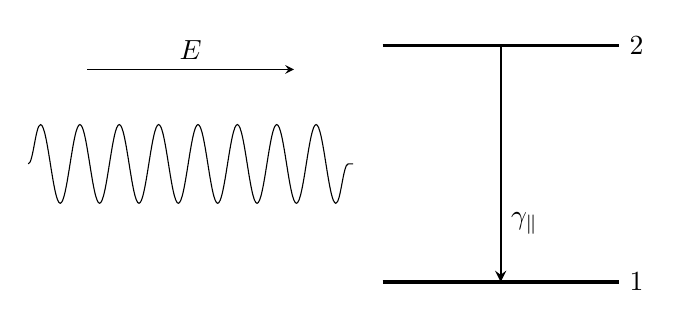
\begin{tikzpicture}[scale=1.5]
  % -- Draw quantum system. 
  \draw[very thick] (0,0) -- (2,0) node[right] {$\Ket{1}$};
  \draw[very thick] (0,2) -- (2,2) node[right] {$\Ket{2}$};
  \draw[thick,->,>=stealth] (1,2) -- (1,0) node[near end,right] {$\gamma_\parallel$};
  
  % -- Draw incoming light.
  \draw[decorate,decoration={snake,amplitude=0.5cm,segment length=0.5cm}] (-3,1) -- (-0.25,1);
  \draw[->,>=stealth] (-2.5,1.8) -- (-.75,1.8) node[midway,above] {$\bo{E}$};
 \end{tikzpicture}
 \end{center}
 \caption[Pictorial representation of the quantum gain medium]
	 {Pictorial representation of the interaction between the
	 quantum gain medium and the incoming field. The quantum system has 
	 two levels, the wavefunction being either $\Ket{1}$ or $\Ket{2}$. The relaxation
	 rate from level 2 to level 1 is given by $1/\gamma_\parallel$.}
 \label{fig:active.salt.twoLevelSystem}
\end{figure}

Solving Schrödinger's equation for a ``bare'', i.e. non-interacting
two-level system yields
  \begin{equation}
   H_0\Ket{j}=\omega_j\Ket{j}	\qquad j=1,2
  \end{equation}
and corresponding eigenfunctions $\Ket{1}$ and $\Ket{2}$. 
The incoming light field acts as a perturbation and source of energy
that stimulates a population transfer from level 1 to level 2 decaying
at a rate $1/\gamma_\parallel$. The perturbation can be written as
  \begin{equation}
   H_1 = e\bo{\mu}\cdot\bo{E}
  \end{equation}
where $e$ is the electric charge and $\bo{\mu}$ is the 
dipole moment tensor of the material.  We expand the solution 
of the perturbed system in the states of the unperturbed system
  \begin{equation}
   \Ket{\psi_1(t)}=C_1(t)\Ket{1}+C_2(t)\Ket{2}
  \end{equation}
and form the density matrix
  \begin{equation}
   \rho(t) = \Ket{\psi_1(t)}\Bra{\psi_1(t)}.
  \end{equation}
It allows us to solve the problem for an ensemble
of two-level systems \cite{GE2010b}.
Using the well-known evolution equations of the density
matrix \cite[\S6.2]{BOY2008} and defining
$D=\rho_{22}-\rho_{11}$, the population difference between the two
levels,  we obtain the equations
\cite[\S5.3]{HAK1985b}
  \begin{align}
   \dot{\bo{P}}^{NL}	&= -\left(i\omega+\gamma_\perp\right)\bo{P}^{NL}+\frac{g^2}{i\hbar}\bo{E}D	\\
   \dot{D}				&= \gamma_\parallel\left(D_0-D\right)-\frac{2}{i\hbar}\bo{E}\cdot\bo{P}^{NL}
  \end{align}
where $g^2$ is the dipole moment of the system, 
$\gamma_\perp$ is an \textit{ad hoc} phenomenological damping
term that comes from the interaction of the ensemble of two-level systems\footnote{The author surmises that it 
could be computed with a mean field approximation.}
and $D_0$ is the equilibrium population. The approach 
uses a \gls{rwa}, but, contrary 
to most derivations, does not invoke the \gls{svea}. 
One of the main approximations, one that is necessary to make
ground, is the \gls{sia}, i.e. $\dot{D}=0$. Writing the fields
as Fourier series
	\begin{align*}
		\bo{P}^{NL}	&= \sum_{\mu}\bo{p}_\mu e^{-ik_\mu t}	&	\bo{E}	&= \sum_{\mu} \bo{\Psi}_\mu e^{-ik_\mu t}
	\end{align*}
leads to the relationship\footnote{We have skipped some steps. See \cite[\S2.2]{GE2010b} for details.}
  \begin{equation}
   \bo{p}_\mu = \frac{g^2}{\hbar}\frac{1}{k_\mu-k+i\gamma_\perp}\frac{D(\bo{r})}{1+\sum\frac{4g^2}{\gamma_\perp\gamma_\parallel}\Gamma(k_\mu)\left|\Psi_\mu(\bo{r})\right|^2}\bo{\Psi}_\mu(\bo{r}).
  \end{equation}
In the TM polarization, this leads to the equation
  \begin{equation}
   \left[\nabla^2+k^2\left(\epsilon(\bo{r})+\frac{g^2}{\hbar}\frac{1}{k_\mu-k+i\gamma_\perp}\frac{D(\bo{r})}{1+\sum_\mu\frac{4g^2}{\gamma_\perp\gamma_\parallel}\Gamma(k_\mu)\left|\Psi_\mu(\bo{r})\right|^2}\right)\right]\Psi_\mu(\bo{r})=0
  \end{equation}
where
	\begin{equation}
		\Gamma(k_\mu) = \frac{\gamma_\perp^2}{(k-k_\mu)^2-\gamma_\perp^2}
	\end{equation}
$\Psi_\mu(\bo{r})$ is the longitudinal component of the field. 

\paragraph{Constant-flux States and Threshold Lasing Modes}
The derivation above, novel to SALT and slightly more accurate
than the standard derivations \cite{GE2010a,GE2010b,EST2013}, shows
that the effect of the quantum gain medium can be modeled as an extra
term in the refractive index in the TM polarization, but leads to an altogether
different differential equation in the TE polarization. To the author's knowledge,
this is never specifically addressed in the SALT articles. 
In the following, we will also focus on the
TM polarization. 

The central feature of \gls{salt} is the introduction of the constant-flux (CF)
states, which are defined by
	\begin{subequations}
	\begin{align}
		\left[\nabla^2+\epsilon(\bo{r})K^2(k)\right]\psi(\bo{r})	&=	0	& \bo{r}\in\mathcal{C}		\label{eq:active.salt.cfCavity}\\
		\left[\nabla^2+\epsilon(\bo{r})k^2\right]\psi(\bo{r})		  &=	0	& \bo{r}\notin\mathcal{C}	\label{eq:active.salt.cfOutside}
	\end{align}
	\end{subequations}
where $\mathcal{C}$ is the cavity region. Inside $\mathcal{C}$, 
the frequency $K(k)$ is allowed to be complex, but outside the cavity
we force $k$ to be real. This allows us to bestow physical meaning
unto the CF states, as they do not suffer from the exponential
growth of the QB states. Despite the non-linearity of the equations, 
the CF states can be used as a basis for the laser modes, and can even 
take into account saturation, spatial hole burning and non-uniform
pumps through the 
	\begin{equation*}
		\frac{D(\bo{r})}{1+\sum_\mu\frac{4g^2}{\gamma_\perp\gamma_\parallel}\Gamma(k_\mu)\left|\Psi_\mu\right|^2}
	\end{equation*}
term. If we restrict our analysis to near-threshold modes, where the lasing field intensity
is very low,  we can neglect the interaction between the different modes. This allows us
to entirely neglect the summation from the previous term
and, writing the pump profile as a pump strength multiplied by a shape function $D(\bo{r})=D_0F(\bo{r})$, 
we obtain
	\begin{align}
		\label{eq:active.salt.tlms}
		\left[\nabla^2+k^2\left(\epsilon(\bo{r})+\frac{\gamma_\perp D_0F(\bo{r})}{k_\mu-k+i\gamma_\perp}\right)\right]\psi(\bo{r}) &=0 & \bo{r}\in\mathcal{C}
	\end{align}
where now the fields and the pump strength are dimensionless parameters measured in units of 
$e_c = \hbar\sqrt{\gamma_\parallel\gamma_\perp}/(2g)$ and 
$D_{0c}=\hbar\gamma_\perp/(4\pi g^2)$, respectively. 
Notice that $\gamma_\parallel$ does not appear explicitly in our set of equations; 
it has become a mere scaling factor \cite[p.~19--20]{GE2010b}.
The solutions of this equation describe the lasing action near lasing thresholds, the threshold lasing modes (TLMs). 
In the case of uniform pumping, i.e. $F(\bo{r})=1$,
the CFs are in a one-to-one correspondence with the TLMs, as we can see by comparing
\eqref{eq:active.salt.cfCavity} and \eqref{eq:active.salt.tlms}. To find
the TLMs, one needs to compute the CF states, find the values of $K^2(k)$ and
infer the values of $D_0$. When the exterior frequency $k$ is such that $D_0$
is real, the resulting couple $(k_a, D_0^a)$ reveals the frequency and threshold
of the lasing mode. This was done in \cite{GAG2014a}. 

However, we will mostly be interested in the case of non-uniform pumping
and/or inhomogeneous refractive index distribution. To find the couple
$(k_a,D_0^a)$, we must solve \eqref{eq:active.salt.tlms} self-consistently
for a real value of $D_0$ such that a pole of scattering matrix hits 
the real $k$-line. In the following, we develop a method that allows
us to compute the \gls{sMatrix} for complex potentials.

\subsection{Numerical Method II: Lippmann-Schwinger}
%\paragraph{Variable Phase Method}
%This elegant method has its roots deep in the literature of quantum-mechanical
%scattering. It is based on the fact that, for central potentials, the 
%\gls{sMatrix} is diagonal and that its elements can be written as
%$e^{i\delta_k}$, where $\delta_k$ is the phase shift suffered by the 
%$k$th partial wave. One can thus find a first order, non-linear differential
%equation \cite{CAL1967} for each $\delta_k$. The method transforms the \gls{bcp} to an \gls{ivp}, as the phase shift
%is bounded. In our present case, the potential is not a central one and the
%\gls{sMatrix} is not diagonal. We will need to solve a coupled system 
%of differential equations to represent the coupling between the different
%partial waves. The \gls{vpm} will give rise to an \gls{ivp} matrix \gls{ode}.
%
%The initial motivation for the use of \gls{vpm} was the computation 
%of the field inside the scatterer. In the \gls{sqa}, modifying 
%the linear algebra operations of the reduction phase yields
%an algorithm that computes the field from given $\bo{A}$ and $\bo{B}$
%coefficients. It is unfortunately highly unstable, to the point 
%of being unusable. The authors of \cite{FOR2012} suggested that
%the \gls{vpm} was stable, suggesting its use over the onion
%discretization of \gls{sqa}. While the \gls{vpm} has some inherent
%issues and our implementation is far from complete, we present
%here the main development both for the interested reader and for 
%future reference. 
%
%The method starts with the angular momentum expansions
%  \begin{subequations}
%  \begin{align}
%   H_z(r,\theta)	&= \frac{1}{\sqrt{2\pi}}\sum_{m=-\infty}^\infty \frac{1}{\sqrt{r}}\psi_m(r)e^{im\theta}	\\
%   n(r,\theta)		&= \frac{1}{\sqrt{2\pi}}\sum_{m'=-\infty}^\infty n_{m'}(r)e^{im'\theta}.
%  \end{align}
%  \end{subequations}
%Substituting these expansions in Helmholtz's equation and projecting
%onto the eigenstate 
%	\begin{equation*}
%		\sqrt{r}e^{-im''\theta}/\sqrt{2\pi}
%	\end{equation*} 
%yields a system of coupled \glspl{ode} for each moment of the field $\psi_m$
%	\begin{equation}
%		\label{eq:active.vpm.equation}
%		\bo{\psi}''-\frac{\mat{M}^2-\mat{I}/4}{r^2}\bo{\psi}+\frac{k^2}{2\pi}\mat{N}^2\bo{\psi}=0
%	\end{equation}
%where 
%	\begin{equation*}
%		\left[\mat{N}(r)\right]_{mm''}=\sum_{m'}n_{m'}(r)\delta_{m+m',m''}.
%	\end{equation*}
%Notice that the free case is recovered when $n(r,\theta)=1$, as 
%then $n_{m'}=\delta_{m'0}$ and 
%	\begin{equation}
%		\bo{\psi}''-\frac{\mat{M^2}-\mat{I}/4}{r^2}\bo{\psi}+k^2\bo{\psi}=0
%	\end{equation}
%a system of uncoupled Bessel equations. At this point, we 
%introduce the matrix \gls{ode}, i.e. \eqref{eq:active.vpm.equation} with as many 
%rows as columns. Each column solves the ODE, but has different boundary conditions
%\cite[\S15.2]{NEW1982}. Since the scattering solution must obey Sommerfeld's radiation
%condition, we use the factorization
%	\begin{equation}
%		\bo{\psi} = \mat{G}_k(r)\mat{W}^{+}(kr)
%	\end{equation}
%where $\left[\mat{W}^{\omega}(kr)\right]_{mm''}=H_m^{(\omega)}(kr)\delta_{mm''}$.
%Outside the \gls{lss}, the solution must be $\mat{W}^+(kr)$. In the general potential
%scattering theory, the \gls{lss} is usually a sphere at infinity, which yields the 
%initial value conditions
%	\begin{align}
%		\mat{G}_k(\infty)	&=\mat{I}	&	\mat{G}_k'(\infty)=\mat{0}.
%	\end{align}
%with 
%	\begin{equation}
%		\mat{G}_k''+2\mat{G}_k'\frac{d\log\mat{W}^\omega}{dr}+\frac{1}{r^2}\left[\mat{G}_k,\mat{M}^2-\mat{I}/4\right]
%					+\frac{k^2}{2\pi}\left(\mat{N}^2-2\pi\mat{I}\right)=0.
%	\end{equation}
%
%The $\mat{G}_k(r)$ matrix represents the phase shifts accumulated by each partial wave $m$ 
%and caused by the $m'$th angular moment of the potential. The factorization procedure 
%effectively transforms the \gls{bcp} to an \gls{ivp}, with the data provided on the 
%\gls{lss}. The matrix ODE can thus be solved by using any good integration routine\footnote{Although
%make sure you use a stiff equation solver. See Appendix \ref{sec:app.numTools.vpm} for details.}.
%
%The scattering matrix of the problem can also be obtained if we 
%compute the conjugate solution, solving with the incoming radiation $\bo{\psi}=\mat{G}_{-k}\mat{W}^-(kr)$
%instead of the outgoing one. The physical wave function is thus given by 
%	\begin{equation}
%		\bo{\psi} = \mat{G}_{-k}(r)\mat{W}^-(kr)+\mat{G}_k(r)\mat{W}^+(kr)\mat{S}_k(k).
%	\end{equation}
%Using the finiteness condition of the field at origin, we have
%	\begin{equation}
%		\mat{S}_k = -\lim_{r\rightarrow0}\mat{W}^{+}(kr)^{-1}\mat{G}_k^{-1}(r)\mat{G}_{-k}(r)\mat{W}^-(kr).
%	\end{equation}

Seeing the differential methods fail, the author of this essay, 
then on the brink of despair, first took notice of the 
power of integral methods. Simply rewriting Helmholtz's 
equation as
  \begin{equation}
   \left[\nabla^2+n_0^2(\omega)k^2\right]\psi=-k^2\Delta n^2(\bo{r};\omega)\psi
  \end{equation}
where 
  \begin{equation}
  	\Delta n^2(\bo{r};\omega)=n_c^2(\bo{r};\omega)-n_0^2(\omega)
  \end{equation}
where $n_c^2(\bo{r};\omega)$ is the permittivity profile of the scatterer
and $n^2_0(\omega)$ the constant permittivity of the environment, or background.
This allows to write a formal solution using the Green's function of Helmholtz's equation
  \begin{equation}
  	\label{eq:active.vpm.fredholmEqn}
  	\psi(\bo{r}) = \phi(\bo{r}) - k^2\mathop{\iint}_\mathcal{C}G_{+}(\bo{r},\bo{r}')\Delta n^2(\bo{r}';\omega)\psi(\bo{r}')d^2\bo{r}'
  \end{equation}
where $\phi(\bo{r})$ is a solution of the homogeneous problem and
  \begin{equation}
  	G_\omega(\bo{r},\bo{r}') = -\frac{i}{4}H_0^{(\omega)}(kn_0|\bo{r}-\bo{r}'|).
  \end{equation}
While \eqref{eq:active.vpm.fredholmEqn} is very general (it can be applied to 
any $\Delta n^2(\bo{r};\omega)$, even to non-linear ones),
the method of solution we will use restricts us to linear problems.

Instead of a \gls{pde}, we now must solve an implicit 
integral equation for the field. It is a Fredholm 
equation of the second kind with a weakly singular, compact
operator. This ensures the existence
and uniticity of the solution \cite{GOH1981,COL2013}.
We solve the surface integral equation in real space by meshing
the cavity $\mathcal{C}$. The details of the meshing is left to 
Appendix \ref{sec:app.numTools.lippmannSchwinger}. Let us denote the set
of cells of our mesh by $\Delta$. We can thus cast the integral
equation as
	\begin{equation}
		\psi_j = \phi_j -k^2\sum_{j'\in\Delta} G_{jj'}\Delta\epsilon_{j'}A_{j'}\psi_{j'}
	\end{equation}
where $\psi_j=\psi(\bo{r}_j)$ and similarly for the other quantities and 
where $A_j$ is the area of cell $j$.  We can
rewrite this as the matrix problem\footnote{This, of course, only holds if the
kernel is linear.} 
	\begin{equation}
		\left(\mat{I}+\mat{K}\right)\bo{\psi}=\bo{\phi}.
	\end{equation}
where 
	\begin{equation}
		K_{jj'} = G_{jj'}\Delta\epsilon_{j'}A_{j'}.
	\end{equation}

The matrix equation is then solved using any good 
linear algebra solver. This yields values for the
field inside the scatterer. The integral equation
is then explicit for the field outside the scatterer. 
Our interest, however, still lies in the computation
of the scattering matrix. It turns out that, if we
use 
	\begin{equation}
		\phi = J_M(kr)e^{iM\theta}
	\end{equation}
as the ``incoming'' field, one may find that the scattering
matrix can be computed via
	\begin{equation}
		S_{Mm} = \delta_{Mm} - \frac{ik^2}{2}\mathop{\iint}_\mathcal{C}e^{-im{\theta'}}J_m(kr')\Delta\epsilon(\bo{r}')\psi^{(M)}(\bo{r}')d^2\bo{r}'.
	\end{equation}
In Appendix \ref{sec:app.numTools.lippmannSchwinger}, we lay out the method in more detail, 
discuss the numerical implementation and present a generalization for the complete 
vectorial electromagnetic fields.

\subsection{Examples}
To demonstrate the method, we compute a lasing mode
of the homogeneous, circular cavity laser. We take $k_\mu=9.25$
and $\gamma_\perp=0.125$ and compute the threshold of a particular
lasing mode. This is done by following the upwards movement 
of the poles of the scattering matrix as $D_0$ is increased.
We show the determinant of the \gls{sMatrix} of the system 
for $D_0=0.027$ in Figure \ref{fig:active.salt.detSmat}.
There is a lasing mode at $k=9.37343358$. It has a low lasing threshold mainly 
because of the extremely high $Q$-factor of its related QB state \cite{GAG2014a}. 

While we see that one of the poles has moved directly 
onto the real $k$-axis and is therefore a physical lasing
mode, perhaps the most striking feature of the pole structure
is the movement of the other poles (contrast with Figure \ref{fig:passive.formalism.symmetrySmatrix}). 
As we had predicted in section on the properties of the \gls{qMatrix} (p.~\pageref{sec:passive.formalism.SpoleStructure}), 
the poles are still symmetric, but along a curve in the complex 
$k$-plane rather than along the real $k$-line. Although it is difficult to derive the exact
form of the curve, we can see that it is of Lorentzian shape, 
as is the imaginary part of the refractive index. Notice also
the clustering of zeros and poles at $k=9.25$, the centre of the
gain transition. This is where the refractive index change is the highest.

\begin{figure}
	\centering
	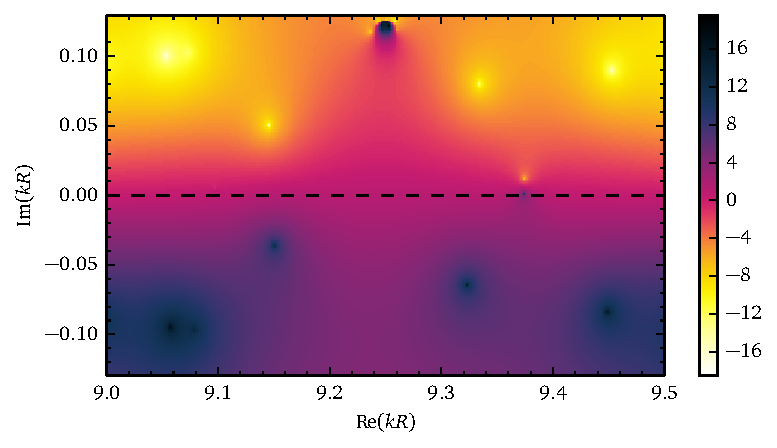
\includegraphics{figs/active/determinantSmatrixSALT.pdf}
	\caption[Map of the determinant of the $\mat{S}$-matrix of the
			amplified system]
			{Map of the determinant of the $\mat{S}$-matrix of the 
			homogeneous, circular cavity laser. We have used $n_c=3.2$, $n_o=1$ and
			$R_0=1$. The gain transition parameters are $\gamma_\perp=0.125$ and $k_\mu=9.25$. 
			This yields a threshold of $D_0=0.027$ for the mode at $k=9.37343358$.}
	\label{fig:active.salt.detSmat}
\end{figure}

\section{Smart Textile Antennae}
The last part of this essay recounts the author's contributions
in a project involving the design and theoretical characterization
of fibre-antennas. This section departs a little from the more theoretical
and numerical musings of the others and presents both the modeling of the 
antennae and their experimental characterization.   

The goal of the original project was to develop an antenna that is compatible with 
WiFi standards (i.e. emits at $f=2.45\,\unit{GHz}$) and can be easily integrated
to textile. These two requirements impose multiple restrictions on both
the materials that can be used and the geometry of the antenna. For instance, 
we would like the antenna to be spun directly into the textile as to have, 
so to speak, a seamless integration of the antenna.

Most solutions today merely affix a patch antenna to a less 
encumbered part of the textile \cite{CAT2004,JAI2013}, e.g. 
on the shoulder pads of a shirt or the front of a t-shirt.
A metallic plate shields the user from the electronic components 
of the patch antenna. Because the properties of patch antennas are
well known \cite{ELL2003}, very little engineering is required and this solution
is thus quite cheap\footnote{The general availability of consumer-grade ``smart''
textile on the Web should suffice to prove this point.}. However, integration 
with the textile is far from seamless, as it is very apparent to the
user that he has become a giant walking antenna. Our project thus 
strives to find antenna designs that have emission properties
as flexible as a patch antenna's while improving textile integration
as to make it transparent to the user.

The concept of a fibre-antenna rapidly established itself
as an ideal solution in our research group, as it provides a rich
architecture upon which to build. A fibre-antenna has the potential
of having good mechanical properties, of shielding the electronic
components from both the user and the washing machine and 
can be loaded directly unto the spools that deliver textile to industrial 
looms, making it both easy to manufacture and transparent to the user.

Before showing the details of our contribution, 
we will first show the important quantities when
working with antennas, and more importantly the design
parameters.

\subsection{Basic Antenna Theory}
Even today, a full 140 years after the publication of 
Maxwell's seminal \textit{Treatise on Electricity and Magnetism}, 
the electromagnetic modeling of radiating structures 
is an ongoing research problem. The notorious difficulty 
of solving Maxwell's equations seriously hampers analytical efforts
and, due to the nature of electromagnetic radiation, numerical
progress is not easier to achieve.

In what follows, we present the Stratton-Chu equations, 
a rigorous solution of Maxwell's equations which relates 
the electric and magnetic fields to the currents and charges 
that ``produce'' them. They can alternatively compute the fields
in all space if they are known on any given surface(s).

\subsubsection{Stratton-Chu Solution}
In antenna problems, we want to compute the field values as a function of 
the sources that contribute to these fields. From electrostatics, we know 
that a current density $\bo{J}$ gives rise to an electric field and a charge 
density $\rho$ gives rise to a magnetic field. In the time-varying picture, 
the electric and magnetic fields become coupled and we take the viewpoint that
the $\bo{J}$ and $\rho$ give rise to both electric and magnetic fields. 

To compute the field from these sources, which are presupposed to exist, 
we must use the Stratton-Chu integrals. The derivation is standard, so we 
refer to \cite{ELL2003}. Consider a volume $V$ of free space containing
sources and possibly excluded sub-volumes $V_i$ bound by surfaces $S_i$ that contain matter
of some kind. By the use of Green's and Stokes' theorems and other vectorial 
identities, we find that the field outside the excluded sub-volumes
can be expressed as
	\begin{subequations}
  \begin{align}
   \bo{E} &= \frac{1}{4\pi}\mathop{\iiint}_V \left(\rho\nabla G+i\omega G\bo{J}\right)dV
	+\frac{1}{4\pi}\oiint_{S_1,\cdots,S_N}\left[\bo{n}\cdot\bo{E}\nabla G+(\bo{n}\times\bo{E})\times\nabla G+i\omega G(\bo{n}\times\bo{H})\right]dS\label{eq:active.antennae.strattonChuE}\\
  \bo{H} &= \frac{1}{4\pi}\mathop{\iiint}_V \bo{J}\times\nabla G dV
	+\frac{1}{4\pi}\oiint_{S_1,\cdots,S_N}\left[-i\omega G(\bo{n}\times\bo{E})+(\bo{n}\times\bo{H})\times\nabla G+(\bo{n}\cdot\bo{H})\nabla G\right]dS\label{eq:active.antennae.strattonChuH}
  \end{align}
where $G$ is the Green's function of the problem
  \begin{equation}
   G(\bo{r},\bo{r}') = \frac{e^{ik|\bo{r}-\bo{r'}|}}{4\pi|\bo{r}-\bo{r}'|}.
  \end{equation}
	\end{subequations}

These two equations are rigorous solutions of Maxwell's equations. 
They can be used with any antenna and provide ways to compute the 
current distribution if it is unknown (constitutes an integral equation in the current\footnote{
This is the basis of the popular computational method known as the \textit{method of moments}
\cite[\S7.5]{ELL2003}.})
and can be used to compute the far-field of antennae when either 
(i) the current distribution is known or (ii) the near-field around the antenna
is known. 
These two properties discriminate antennae into two categories, denoted Type I and Type II.

Type I antennae have a well-approximated current distribution, which means that there are no
sub-volumes to be excluded and therefore no surface integrals in expressions 
\eqref{eq:active.antennae.strattonChuE} and \eqref{eq:active.antennae.strattonChuH}. 

On the other hand, Type II antennae have well-approximated near-fields, leading
us to exclude the volume containing the antenna. Expressions \eqref{eq:active.antennae.strattonChuE}
and \eqref{eq:active.antennae.strattonChuH} contain only surface integrals, then.

We will give examples relating these two types of antennae to the 
Stratton-Chu equations when we have defined the antenna parameters.

\subsubsection{Antenna Parameters}
In the design of our antenna, we will want to optimize the value
of some parameters. We will now describe some of these parameters.

\paragraph[Directivity and Gain]{Directivity and Gain \cite[\S 1.16]{ELL2003}}
Given a radiation pattern measured (in the far-field) as the power density 
$\mathcal{P}(\theta,\varphi)$, we can define its \textit{directivity}
as
  \begin{equation}
   D(\theta,\varphi) = \frac{4\pi\mathcal{P}(\theta,\varphi)}
			{\int_0^\pi\int_0^{2\pi}\mathcal{P}(\theta',\varphi')\sin\theta'd\theta'd\varphi'}.
  \end{equation}
The value of the directivity is less than unity if the power density radiated at angle $(\theta,\varphi)$
is less than the average power radiated. For instance, an isotropic antenna will possess a unit directivity
for all angles while a highly directional antenna will have a sharp peak  in its directivity function 
at some angle $(\theta^*,\varphi^*)$.

Another interesting concept to introduce is \textit{partial directivity}. 
The power density can be divided into two contributions: the $\theta$-
and $\varphi$-polarized contributions and we can write
  \begin{equation}
    \mathcal{P}(\theta,\varphi) = \mathcal{P}_\theta(\theta,\varphi)+\mathcal{P}_\varphi(\theta,\varphi)
  \end{equation}
where the subscripts indicate the polarization state. The partial 
directivities hence follow
  \begin{equation}
   D(\theta,\varphi) = D_\theta(\theta,\varphi)+D_\varphi(\theta,\varphi).
  \end{equation}

We can also introduce the gain, which characterizes the loss
and the directivity of the antenna simultaneously. It is simply given
as
  \begin{equation}
    G(\theta,\varphi) = \frac{4\pi r^2\mathcal{P}(\theta,\varphi)}{P}
  \end{equation}
where $P$ is the power fed into the antenna. Because of the 
losses, 
	\begin{equation*}
		P/r^2\geq\int_0^\pi\int_0^{2\pi}\mathcal{P}(\theta',\varphi')\sin\theta'd\theta'd\varphi'
	\end{equation*}
such that $G(\theta,\varphi)\leq D(\theta,\varphi)$. 

We can also define partial gains in the exact same fashion we defined partial
directivities.

Radiation efficiency $\eta$ is defined as the ratio of the total radiated power 
to the power accepted by the antenna \cite{IEEE145-1993}.

	\begin{exmp}[Dipole Antenna \cite{ELL2003}]
		Perhaps the most basic antenna design, it has the form shown in 
		Figure \ref{fig:active.antennae.dipoleAntenna}. 
		
				\begin{figure}
					\begin{center}
					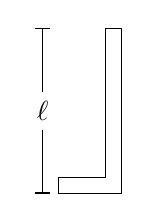
\begin{tikzpicture}
						\draw (-0.7, 0.1) -- (-0.1, 0.1) -- (-0.1,2) -- (0.1,2) -- (0.1,-0.1) -- (-0.7,-0.1) -- cycle;
						\draw[|-|] (-0.9,-0.1) -- (-0.9,2) node[midway,fill=white] {$\ell$};
					\end{tikzpicture}
					
					\vspace{0.1cm}
					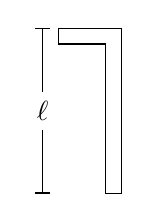
\begin{tikzpicture}[yscale=-1]
						\draw (-0.7, 0.1) -- (-0.1, 0.1) -- (-0.1,2) -- (0.1,2) -- (0.1,-0.1) -- (-0.7,-0.1) -- cycle;
						\draw[|-|] (-0.9,-0.1) -- (-0.9,2) node[midway,fill=white] {$\ell$};
					\end{tikzpicture}
					\end{center}
					\caption[Geometry of the dipole antenna]
							{Geometry of the dipole antenna. It consists of a pair of thin
							wires whose diameters are much smaller than their length $\ell$.
							They are actually separated by an infinitesimal spacing. It has
							been made visible for the drawing. Current is fed to the antenna
							from one of the incoming wires. The $z$-coordinate has its origin
							directly between the two wires.}
					\label{fig:active.antennae.dipoleAntenna}
				\end{figure}
		
		\noindent It is also called the
		slender dipole antenna, as we consider the limit where the diameter of
		the wire is much smaller than the wavelength, making the dipole antenna
		a 1-dimensional problem. The current flowing through the dipole can be
		approximated by 
			\begin{equation}
				I(z) = I_m\sin\left[k(\ell-|z|)\right]
			\end{equation}
		where $I_m$ is the intensity of the current.
		It is thus categorized as a Type I antenna. We can use the volumetric part
		of the Stratton-Chu solution to compute the far-field of such antennae. Introducing
		a directional weight function $\mathcal{A}_{\{\theta,\varphi\}}$ such that
			\begin{equation}
				\mathcal{P}_{\{\theta,\varphi\}}(\theta,\varphi) = \left|\mathcal{A}_{\{\theta,\varphi\}}\right|^2
			\end{equation}
		and using the far-field approximation of the Green function in Stratton-Chu's equation, we obtain
			\begin{equation}
				\mathcal{A}_\theta(\theta) = -I_m\sin\theta\int_{-\ell}^\ell\sin\left[k(\ell-|z|)\right]e^{ikz\cos\theta}dz
			\end{equation}
		which can be integrated to yield
			\begin{equation}
				\mathcal{A}_\theta(\theta) = -\frac{2I_m}{k\sin\theta}\left[\cos(k\ell\cos\theta)-\cos(k\ell)\right].
			\end{equation}
		This is the functional form of the field on the azimuthal great circle as the radius of the sphere goes
		to infinity.  Figure \ref{fig:active.antennae.dipoleFarField} shows a cross-section of the 3D far-field
		along any $\varphi$ for the half-wave dipole antenna ($\ell=\lambda/4$).
		
		\begin{figure}
			\centering
			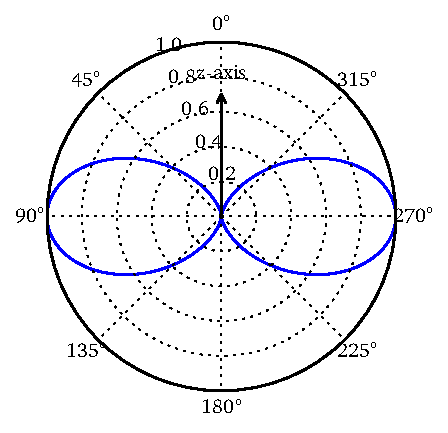
\includegraphics{figs/active/farField-dipole.pdf}
			\caption{Cross-section of the 3D far-field of the half-wave dipole antenna.}
			\label{fig:active.antennae.dipoleFarField}
		\end{figure}
	\end{exmp}
	
		\begin{exmp}[Near- to Far-Field Transformation]\label{ex:active.antennae.nearToFarTrans}
			If, instead of knowing the currents and charges in a given volume $V$, we know the 
			fields on the boundaries $S_i$ of a given number of volumes $V_i$ in which there (supposedly) exist
			unknown charges and currents producing those fields, we can use the boundary terms in the Stratton-Chu
			equation to compute the field outside the antenna. This often arises when using \gls{fem}
			and \gls{fdtd} software, as both methods solve the fields in a given computational volume. The
			far-field is not directly available to them, as this would require a very large computational volume.
			Usually, then, one can specify a boundary which encloses all scattering objects (the \gls{lss}). 
			Since the fields are known, we can use the surface part of \eqref{eq:active.antennae.strattonChuE}
			together with the far-field expansion of $G(\bo{r},\bo{r}')$ to compute the far-field via a simple
			quadrature of the near-field. For instance, this is how the commercial software COMSOL computes the
			far-field.
			
			In our previous example, we could define the \gls{lss} as the cylinder enclosing
			the whole of the dipole antenna. The Stratton-Chu integrals can then be evaluated 
			with the known field on the cylinder and yield the far-field. 
			\end{exmp}
	

\paragraph{Scattering Parameters}
The scattering parameters (or $S$-parameters) are
usually defined through a linear $N$-port network. 
Suppose we have an electronic device comprising
$N$ ports, or points of entry. Imagine shining light onto, 
or make a current flow into,
one of the ports, say port $j$. A certain percentage
of the power carried by this light/current be reflected 
by this port and the rest will be transmitted to the
other ports or absorbed in the medium. The \textit{reflection}
coefficients are given by $S_{jj}$ while the transmission
coefficients are given by $S_{ji}$ ($i\neq j$) where $\mat{S}$
is the scattering matrix of the network. In a reciprocal (in the sense
of Lorentz) network, the scattering matrix will be equal to its
transpose, i.e. $S_{ij}=S_{ji}$. In a lossless network, the scattering
matrix will be unitary. 

\begin{figure}
 \begin{center}
 \begin{tikzpicture}
  % -- Draw the overall shape.
  \draw[very thick] (0,0) -- (8,0) -- ++(0,-2) -- ++(-3,0) -- ++(0,-2) -- ++(-2,0) -- ++(0,2) -- ++(-3,0) -- ++(0,2); 
  
  % -- We draw the reflected/transmitted arrows.
  \draw[->,>=stealth] (8.25,-0.5) -- ++(1,0) node[near end,above] {$a_1$};
  \draw[<-,>=stealth] (8.25,-1.5) -- ++(1,0) node[near end,above] {$b_1$};
  \draw[<-,>=stealth] (-1.25,-0.5) -- ++(1,0) node[near start,above] {$a_2$};
  \draw[->,>=stealth] (-1.25,-1.5) -- ++(1,0) node[near start,above] {$b_2$};
  \draw[->,>=stealth] (3.5,-4.25) -- ++(0,-1) node[near end,right] {$a_3$};
  \draw[<-,>=stealth] (4.5,-4.25) -- ++(0,-1) node[near end,right] {$b_3$};
 \end{tikzpicture}
 \end{center}
 \caption[Example of a 3-port network]{Example of a 3-port network. The ``ends'' of the structure are generally used at its ports.}
 \label{fig:active.antennae.network}
\end{figure} 

This is, of course, highly reminiscent of the scattering operator
in quantum-mechanical scattering which relates the outgoing (scattered)
components to the incoming (incident) components
  \begin{equation}
   \Ket{\Psi_\text{out}}=\mathcal{S}\Ket{\Psi_\text{in}}.
  \end{equation}
In this case, the ``ports'' are the different angular momenta
components rather than physical input/output connections. 
The precise nature of ports is somewhat arbitrary in optical structures.

\subsection{The Leaky Coaxial Cable}
A standard antenna design, the leaky coaxial cable, or \gls{lcx}, will be the primary 
object of our present study. Its relatively simple design: a coaxial cable from which
some parts of the metal coating are removed as to form ``windows'', made it a safe choice
to toy with both the experimental fabrication procedure and the numerical modeling. 
Usual LCXs are much longer than the wavelength at which they are meant to operate, with 
a unit cell (see Figure \ref{fig:active.antennae.fibre-antenna}) of comparable size.

Our antennae, contrary to typical LCXs, have lengths similar to that of the operating
wavelength. Figure \ref{fig:active.antennae.fibre-antenna.xsection} shows a cross-section of
of a typical LCX antenna and Figure \ref{fig:active.antennae.fibre-antenna.topview} shows
a top view of the fibres our group actually made. They all contain three windows of varying
widths $S_z$ and distance between windows $d_z$, making for fibres having all approximately
$L\sim24\,\unit{cm}$. Table \ref{tab:active.antennae.rfxx-parameters} shows the geometrical parameters
of the fabricated antennae, while Table \ref{tab:active.antennae.physicalParameters} shows the 
physical parameters of the materials involved. 

\begin{figure}
  \centering
  \begin{subfigure}[b]{\textwidth}
    \centering
   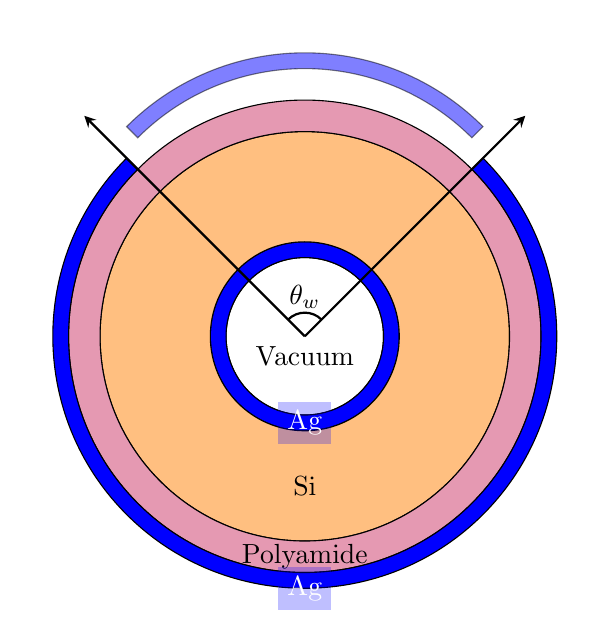
\begin{tikzpicture}
    % -- Draw different materials of the antenna.
    \coordinate (O) at (0,0);
    \draw (O) circle (1);											% Vacuum core
    \draw[fill=blue, even odd rule] (O) circle (1.2) (0:1) arc (0:360:1);					% Silver layer
    \draw[fill=orange!50!white, even odd rule] (O) circle (2.6) (0:1.2) arc (0:360:1.2);			% Dielectric (Si) layer
    \draw[fill=purple!40!white, even odd rule] (O) circle (3) (0:2.6) arc (0:360:2.6);				% Dielectric (polyamide) layer
    \draw[fill=blue,even odd rule] (45:3) -- (45:3.2) arc (45:-225:3.2) -- (-225:3) arc (-225:45:3) -- cycle;	% Second silver layer
    \draw[fill=blue,opacity=0.5,even odd rule,yshift=0.4cm] (45:3) -- (45:3.2) arc (45:135:3.2) -- (135:3) arc (135:45:3) -- cycle;
    
    % -- Draw the angular size of the window.
    \draw[->,>=stealth,thick] (O) -- (-2.8,2.8);
    \draw[->,>=stealth,thick] (O) -- (2.8,2.8);
    \draw[thick] (45:0.3) arc (45:135:.3); 
    \node at (0,0.5) {$\theta_w$};
    
    % -- Place text for materials
    \node at (0,-0.25) {Vacuum};
    \node[text=white,fill=blue,fill opacity=0.25,text opacity=1] at (0,-1.1) {Ag};
    \node at (0,-1.9) {Si};
    \node at (0,-2.8) {Polyamide};
    \node[text=white,fill=blue,fill opacity=0.25,text opacity=1] at (0,-3.2) {Ag};
   \end{tikzpicture}
   \vspace{0.25cm}
   \caption{View of the cross-section: in order of increasing radius, we have: vacuum, silver, silica, polyamide and silver.
	    We have shown a cross-section where there is a ``window''. When there are no windows, 
	    the outer silver layer takes up the entire circumference of the fiber.
	    $\theta_w$ is the angular size of the windows.}
   \label{fig:active.antennae.fibre-antenna.xsection}
  \end{subfigure}
  
  \vspace{4cm}
  
  \begin{subfigure}[b]{\textwidth}
    \centering
   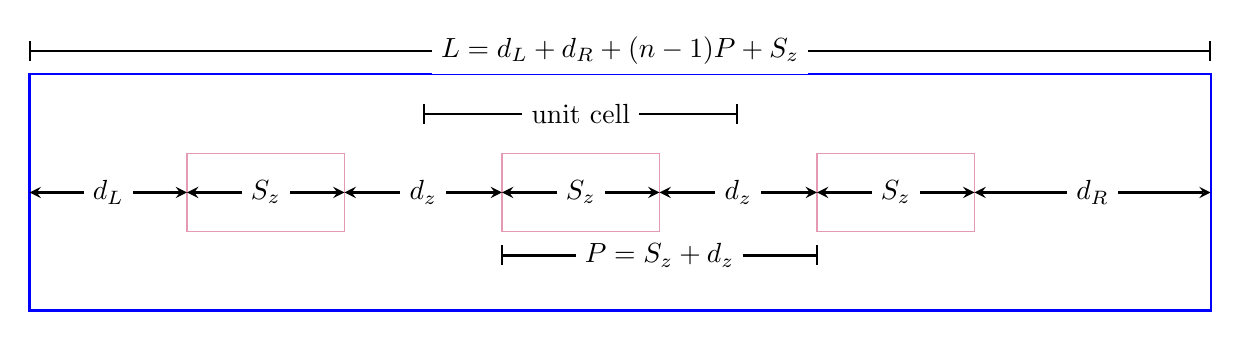
\begin{tikzpicture}
    \draw[blue,thick] (0,-0.5) rectangle (15,2.5);
    \draw[purple!40!white] (2,0.5) rectangle (4,1.5);
    \draw[purple!40!white] (6,0.5) rectangle (8,1.5);
    \draw[purple!40!white] (10,0.5) rectangle (12,1.5);
    
    \draw[<->,>=stealth,thick] (0,1) -- (2,1) node[midway,fill=white] {$d_L$};
    \draw[<->,>=stealth,thick] (2,1) -- (4,1) node[midway,fill=white] {$S_z$};
    \draw[<->,>=stealth,thick] (4,1) -- (6,1) node[midway,fill=white] {$d_z$};
    \draw[<->,>=stealth,thick] (6,1) -- (8,1) node[midway,fill=white] {$S_z$};
    \draw[<->,>=stealth,thick] (8,1) -- (10,1) node[midway,fill=white] {$d_z$};
    \draw[<->,>=stealth,thick] (10,1) -- (12,1) node[midway,fill=white] {$S_z$};
    \draw[<->,>=stealth,thick] (12,1) -- (15,1) node[midway,fill=white] {$d_R$};
    \draw[|-|,thick] (-0.01,2.8) -- (15.01,2.8) node[midway,fill=white] {$L=d_L+d_R+(n-1)P+S_z$};
    \draw[|-|,thick] (5.99,0.2) -- (10.01,0.2) node[midway,fill=white] {$P=S_z+d_z$};
    \draw[|-|,thick] (5,2) -- (9,2) node[midway,fill=white] {unit cell};
   \end{tikzpicture}
   \vspace{0.25cm}
   \caption{Top view: the positions of the windows are usually asymmetric, i.e. $d_L\neq d_R$. The distance between
	    the windows is given by $d_z$ and the length of the windows are $S_z$. We notice that the length of the 
	    fibre is given by $L=d_L+d_R+(n-1)P+S_z$ where $P=S_z+d_z$ is the period between windows and $n$ is the number
	    of windows.}
   \label{fig:active.antennae.fibre-antenna.topview}
  \end{subfigure}
  \caption{Geometry of the fibre-antenna}
  \label{fig:active.antennae.fibre-antenna}
\end{figure}

\paragraph{Modeling \glspl{lcx}}
The modelization of \gls{lcx} is not a new field \cite{DEL1980,WAN2001,KIM2007,ADD2008}.
They have been studied using a variety of analytical and numerical methods. Most of them 
depend on a set of \textit{crucial} approximations that cannot be assumed to hold 
in our particular case:

\begin{description}
	\item [Periodicity of the structure] The $z$-periodicity of the geometry and 
		and material parameters paves the way for a Floquet-Bloch expansion of the 
		fields. This is used in \cite{WAN2001}.
	\item [Narrow slits] A perturbation theory, where slits are supposed to be 
			small as compared to the wavelength, $kS_z\ll1$, is used in \cite{KIM2007}.
	\item [Transmission line behaviour] One of the most important approximation, it stipulates
			that the \gls{lcx} supports a single TEM propagating mode. This allows the 
			unambiguous use of scalar voltages and currents as the physical observables
			\cite{PAU2007}. It also allows
			the use of simpler numerical methods, such as using the overlap between the 
			propagating mode and the radiation continuum to quantify the radiation 
			properties \cite{SHI1989,ADD2008}. 
\end{description}

In our case, the worst offender is the last one, as our metal deposition method
does not allow for a fine control of the thicknesses deposited, nor ensure its
smoothness. The TEM approximation depends on the metal layers behaving almost as 
perfect conductors. Our metallic layers are typically smaller than the skin
depth of the metal, which makes the approximation invalid (we will explore
this later in this essay). 

Moreover, we cannot consider the structure to be periodic, as the total 
length of the fibre-antenna is of the order of the wavelength ($\lambda\sim12\unit{cm}$) and the period
of the slots is smaller than the wavelength. Given the size of the slots, 
the author is comfortable to say that we neither are in the perturbation regime. 
Figure \ref{fig:active.antennae.fibre-antenna} shows the actual design and the important parameters.
We will use the fact that the first radiation harmonics of a \gls{lcx} is giben 
by the relation \cite{WAN2001}
	\begin{equation}
		f_1 = \frac{c}{P\left(\sqrt{\epsilon_r+1}\right)}
	\end{equation}
to guide the numerical modeling.

\paragraph{Specifications of the Devices}
To be able to theoretically investigate the behaviour of these antennas, we must
know their physical and geometrical properties. 
The parameters of the dielectric materials are provided by the manufacturer of the
optical fibres we use as a building platform,
Polymicro Technologies, and are reproduced in Table \ref{tab:active.antennae.modelParameters}.

The thickness of the metallic layers is more delicate and depends on the 
minute details of the deposition method. 
As a first approximation,  we can compute the thicknesses by measuring
the D.C. resistance of the inner and outer layers of silver and
using the relation \cite[p.~204]{CHE1989}
  \begin{equation}
    \label{eq:active.antennae.dcResistivity}
    R = \frac{L}{\sigma A}
  \end{equation}
where $L$ is the length of the fibre, $\sigma$ the conductivity of the silver
layer and $A$ its area. For the inner and outer layers, we have
  \begin{align}
    A_\text{inner}	&= \int_0^{2\pi}\int_{t_\text{vac}-t_\text{Ag1}}^{t_\text{vac}}r\,dr d\theta= \pi\left(2t_\text{vac}t_\text{Ag1}-t_\text{Ag1}^2\right)	\\
    A_\text{outer}	&= \int_0^{2\pi}\int_T^{T+t_\text{Ag2}}r\,dr d\theta = \pi\left(2Tt_\text{Ag2}+t_\text{Ag2}^2\right)
  \end{align}
where $T=t_\text{vac}+t_\text{Ag1}+t_\text{Si}+t_\text{pyamide}$. 
Substituting these results into \eqref{eq:active.antennae.dcResistivity}
yields
  \begin{subequations}
  \label{eq:active.antennae.thickGeneralEquations}
  \begin{align}  
   -t_\text{Ag1}^2 + 2t_\text{vac}t_\text{Ag1}-\frac{L}{\sigma_\text{Ag0}\pi R_\text{inner}}	&=0	\\
   t_\text{Ag2}^2 + 2Tt_\text{Ag2}-\frac{L}{\sigma_\text{Ag0}\pi R_\text{outer}}			&=0
  \end{align}
  \end{subequations}
where the $R$s are the measured D.C. resistances for each shell. 
This can readily be solved using the quadratic equation. Using the bulk conductivity
of silver (see Table \ref{tab:active.antennae.physicalParameters}) yields the
thicknesses found in Table \ref{tab:active.antennae.rfxx-parameters}.

Notice that this assumes smooth metallic layers (no surface inhomogeneities) and
constant conductivity within the whole volume. We will return to this assumption
shortly. 

\begin{table}
  \newcolumntype{d}{D{.}{.}{3}}
  \caption[Geometric and physical parameters of the \gls{lcx} antennae]
	  {Geometric and physical parameters of the \gls{lcx} antennae.
	  Units are repeated from column above if not indicated.}
	\label{tab:active.antennae.modelParameters}
 \begin{subtable}[t]{0.65\textwidth}
 \caption[Geometric parameters of the RF21/RF33 fibre designs]
	  {Geometric parameters of the fibre designs. 
	  The thicknesses of the layers are listed in order, starting
	  from the inner layer to the outer layer of the fibre-antenna.}
 \label{tab:active.antennae.rfxx-parameters}
 \begin{tabular*}{\textwidth}{l@{\extracolsep{\fill}}c@{\extracolsep{\fill}}d@{\extracolsep{\fill}}d@{\extracolsep{\fill}}d@{\extracolsep{\fill}}d}
  \hline\hline
  Quantity			& Unit			& \multicolumn{1}{c}{RF21} 	& \multicolumn{1}{c}{RF27\parnote{Measurements are approximate; values for the inner and outer resistances were lost. We assume they are identical to the RF29.}}	& \multicolumn{1}{c}{RF29}	& \multicolumn{1}{c}{RF33}	\\
  \hline
  $t_\text{vac}$	& $\unit{\mu m}$& 99.874					& 99.900					& 99.646			& 99.924			\\
  $t_\text{Ag1}$	& 				& 0.126						& 0.100						& 0.354				& 0.0766			\\
  $t_\text{Si}$		& 				& 273						& 273 						& 273				& 273				\\
  $t_\text{pyamide}$& 				& 24						& 24 						& 24 				& 24				\\
  $t_\text{Ag2}$	& 				& 0.101						& 0.100						& 0.306				& 0.030				\\
  $d_L$				& $\unit{mm}$	& 27						& 30						& 31				& 30.91				\\
  $d_R$				& 				& 55						& 55						& 55				& 54.72				\\
  $S_{z1}$\parnote{Each window has a different $S_z$ and $d_z$.}
					& 				& 32						& 34						& 33				& 34.36				\\
  $S_{z2}$			& 				& 32						& 34						& 34				& 34.06				\\
  $S_{z3}$			& 				& 32						& 34						& 33.5				& 33.87				\\
  $d_{z1}$			& 				& 28						& 28						& 29				& 27.44				\\
  $d_{z2}$			& 				& 28						& 28						& 28.5				& 28.36				\\
  $L$				& $\unit{cm}$	& 30.0						& 24.3						& 24.4				& 24.372			\\
  $\theta_w$		& $\unit{deg}$	& 180						& 180						& 180 				& 180				\\
  $R_\text{inner}$	& $\unit{\Omega}$& 60.0						& \multicolumn{1}{c}{---}	& 60				& 80.5				\\
  $R_\text{outer}$	&				& 20.0						& \multicolumn{1}{c}{---}	& 20				& 59.8				\\
  \hline\hline
 \end{tabular*}
 \begin{flushleft}
 \parnotes
 \end{flushleft}
 \end{subtable}\hfill
 \begin{subtable}[t]{0.3\textwidth}
  \begin{center}
 \caption{Physical parameters of the materials used in the fibre-antennae.}
 \label{tab:active.antennae.physicalParameters}
 \begin{tabular*}{\textwidth}{l@{\extracolsep{\fill}}c@{\extracolsep{\fill}}d}
  \hline\hline
  Quantity			& Unit			& \multicolumn{1}{c}{Value}		\\
  \hline
  $\epsilon_\text{Si}$		& --			& 3.77		\\
  $\epsilon_\text{pyamide}$	& --			& 3.50		\\
  $\sigma_\text{Ag0}$		& $\unitfrac{MS}{m}$	& 63.0		\\
  $\sigma_\text{AgO0}$		& 			&  6.79		\\
  $\lambda_\text{Ag}$		& $\unit{nm}$		& 40		\\
  \hline\hline
 \end{tabular*}
 \begin{flushleft}
 \parnotes
 \end{flushleft}
 \end{center}
 \end{subtable}
\end{table}

\paragraph{Choice of simulation software}
The LCXs to be modeled have a decidedly complex geometry that
no possess no symmetry and metallic layers of high, though not infinite,
conductivity. To properly take the effects of both situations into account, 
one would need, at the very least, to use multi-scale discretization techniques.
Unfortunately, the extremely wide range in the characteristic sizes of the structures
(from the nanometer to the millimeter) makes meshing the LCX geometry a Herculean, 
if not even Sisyphean, task. 
The issue of meshing thin silvers layers has already been solved in the literature
and involves replacing the silver shells by appropriate boundary conditions \cite{MIT1968}. 

The two requirements discussed above essentially destroy all hope of using any
of the methods we have devised in the last sections of this essay. The eigenbasis
expansions suffer from poor mesh control\footnote{There exists, for instance, 
algorithms that compute the Discrete Fourier Transform for non-uniform
samples, and such endeavors are worthwhile, but their sizable numerical
cost and their only slightly better mesh control is not worth their effort in 
our particular case.}, direct integration Helmholtz's or Maxwell's equations
is usually unstable\footnote{Not always however, as the FDTD method does just that.
It requires, however, some numerical legwork.} and it is notoriously difficult
to incorporate boundary conditions naturally in the framework of the Fredholm 
integral methods \cite{VAN1991,MAR2003}. This leaves us with two choices: the \gls{fdtd}
method and the \gls{fem}. The former can deal with arbitrary boundary conditions
rather easily, but generates a fixed scale mesh \cite{OSK2010}. The latter, by the use of the weak
form of Maxwell's equations, can easily incorporate any type of boundary conditions
and work with multi-scale and even adaptive meshes. We thus use the commercial \gls{fem}
software Ansys HFSS to model the frequency response of the the \gls{lcx} antennae.

The software comes with bundled CAD capabilities. To model the LCXs, we draw a coax 
cable inside a cylinder of larger radius that acts as the ``environment''. Its borders are
terminated by perfectly matched layers, or PMLs \cite{BER1994}, that absorb the field emanating 
from the antenna. They serve to emulate the Sommerfeld radiation condition\footnote{
This type of absorbing boundary conditions has been used for decades and has lead
to a number of problems, which in turn led to a rich literature. It was shown that naïvely using 
PMLs led to spurious solutions \cite{KON1976,KOS1984,KOS1985}. They are usually removed by
adding the null term $\left(\nabla\cdot\bo{H}^*\right)\left(\nabla\cdot\bo{H}\right)$
in the functional that is minimized.
In the microcavities field, specifically in the finding of resonances, it was 
found out that the PMLs caused large errors in the determination of the
imaginary part of the resonant $k$ \cite{HOW1993,HOE1998,BOR2004} The problem
was recently solved for microcavities having azimuthal symmetry \cite{OXB2007,CHE2013}.}
and to ensure that the waves radiated by the antenna are not reflected back to it
from the edges of the computational domain. In a driven problem like ours, some
numerical back-reflections from the PMLs can and do occur, but cause little
to no problem. The metallic layers are implemented as ``Layered Impedance Boundary
Conditions'', which are essentially a generalization to an arbitrary number of
layers of the formalism laid out in \cite{MIT1968}. The ports of the structure
are its left and right coupling points, or simply ``ends.'' Technically, we could
define the windows as open ports, but their frequency response is difficult to 
measure experimentally and consider the light radiating through them as loss 
in the system. In other words, $|\det\mat{S}|<1$. Solving the system boils down
to the definition of the input field on the ports and letting the solver solve
Maxwell's equations in the computational domain. The $S$-parameters correspond
to the fraction of the power that either (i) returned back into the source port
or (ii) traveled all the way to the other port. This is done for both ports in turn. 
The far-field associated with each run is computed via the near- to far-field 
transformation that is discussed in Example \ref{ex:active.antennae.nearToFarTrans}, 
using the environment's boundary as the \gls{lss}.

The traces of the $S$-parameters, i.e. the value of $S_{ij}$ as a function of 
the frequency of the input fields, will be of primary interest. The frequency
response can give information about the quality factor of the resonances, as well as
hinting at specific radiation mechanisms. The analysis below will be divided
in two parts: the analysis of the traces on their own, and comparison with the 
theoretical/simulation traces. Notice that our device is reciprocal, such that
$S_{12}=S_{21}$. We only have three independent scattering parameters to study.

\subsubsection{Analysis of Experimental Traces}
Before showing the correspondence (or lack thereof) between the
simulated and measured traces, we will analyze the traces by themselves
and try to extract any information we can. The main tool 
we will use to do so is the autocorrelation of the traces. It is defined
as 
	\begin{equation}
		c_{XX}(\Delta t) = \frac{\avg{\left[X(t+\Delta t)-\avg{X(t)}\right]\left[X(t)-\avg{X(t)}\right]}}{\avg{X(t)^2}-\avg{X(t)}}
	\end{equation}
for a time series $X(t)$. Since the autocorrelation of a signal has the same periodicity
as the input signal, it is a practical way to reduce the noise of experimental
data and detect periodicity. 

Another interesting property that can be used to theoretically characterize
the type of scattering occurring in our structures is the decay of the 
autocorrelation function. In the 1980s, it was shown that if the underlying
classical mechanics of the structure showed chaoticity, the corresponding
open quantum scattering problem retained the signature of chaos 
through the Lorentzian decay of the autocorrelation of the scattering matrix 
elements \cite{BLU1988,JAL1990}. We will thus use a Lorentzian fit of the form 
	\begin{equation}
		L(x;\bo{p}) = p_0 \frac{p_1/2}{x^2-p_1^2/4}
	\end{equation}
where $\bo{p}$ is a vector of parameters to be fitted. The quality of the
fit will serve as a qualitative way to determine the quality of the
fibre-antenna. A good Lorentzian fit indicates irregularity of the spectral
response and consequently of the bad quality of this particular fibre-antenna
realization. The reasoning is that the resonances (or dips in the traces, rather) are the result
of the commensuration between the geometry and the wavelength of the light and 
are thus expected to repeat periodically. 

\paragraph{RF10}
This is the first realization of the fibre-antenna and, 
consequently, its $S$-parameters are far from the desired
ones (see Figure \ref{fig:active.lcx.rf10sParameters}), as they
show a single dip at $f\sim800\,\unit{MHz}$. The rapid decrease
of the autocorrelation reflects on the poor fabrication process.
In other words, the lengths of the window are so different
that the wave essentially undergoes random motion. 

\begin{figure}[h]
 \centering
 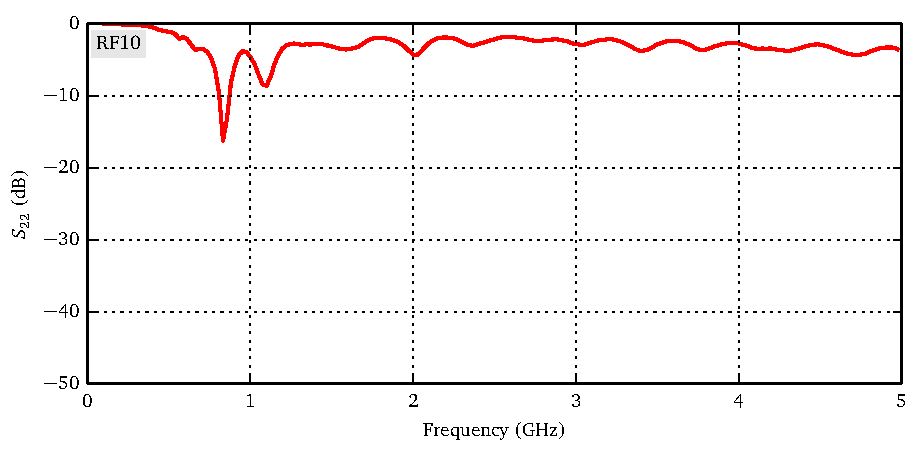
\includegraphics{figs/active/RF10-sParameters.pdf}
 \caption[Experimental $S_{22}$ trace of the RF10 fibre-antenna]
 		{Experimental $S_{22}$ trace for the RF10 fibre-antenna. 
 		The relatively background value of $\sim -4\,\unit{dB}$ indicates
 		that much of the power is reflected back from port 2 (the right-hand side of
 		the antenna, according to our specifications). Also, its single dip at $f\sim800\,\unit{MHz}$
 		is mostly useless for our purposes.}
 \label{fig:active.lcx.rf10sParameters}
\end{figure}

\begin{figure}[h]
 \centering
 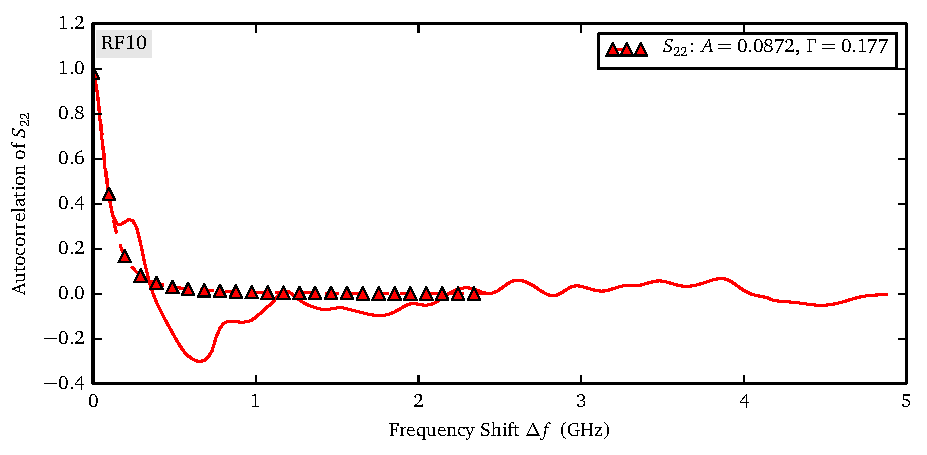
\includegraphics{figs/active/RF10-autoCorrelation.pdf}
 \caption[Autocorrelation of the experimental trace of $S_{22}$ for the RF10 fibre-antenna]
 		{Autocorrelation of the experimental trace of $S_{22}$ for the RF10 fibre-antenna.
 		The dotted line represents the Lorentzian fit. Despite relatively strong negative correlation around $800\,\unit{MHz}$,
 		it is almost zero over the whole interval, but does not fit the Lorentzian.}
 \label{fig:active.lcx.rf10autocorrelation}
\end{figure}

\paragraph{RF21}
The traces of this particular realization shows definite dips, particularly
in the transmission coefficient $S_{12}$, with associated although weaker
dips in both reflection coefficients. The two dips, occurring at $f\sim1.8\,\unit{GHz}$
and $f\sim3.0\,\unit{GHz}$, correspond to optical wavelengths $\lambda_\text{opt}=c/(nf)$ 
of approximately $8.5\,\unit{cm}$ and $5.3\,\unit{cm}$, respectively. They correspond
to the lengths of the first and last scattering cells, approximately; the existence
of these two dips thus seems predicated on the asymmetry of the cells ($d_L\neq d_R$). The fact that all
traces show dips at these frequencies implies that energy is lost in the system. Neglecting
the losses to the metallic layers (they are thinner than the skin depth, minimizing the losses),
we can assume that the lost energy is radiated away through the windows. This design thus 
has two operating frequencies, both outside the desired range, however. 

\begin{figure}[h]
 \centering
 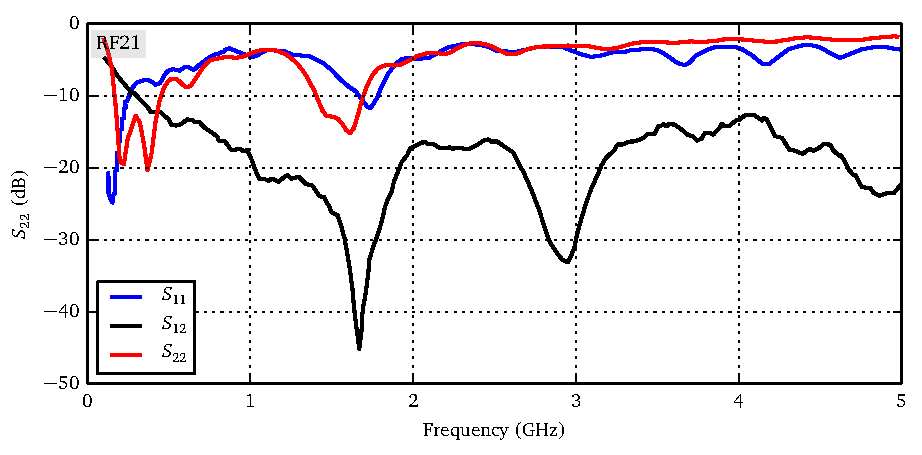
\includegraphics{figs/active/RF21-sParameters.pdf}
 \caption[Experimental $S_{22}$ trace for the RF21 fibre]
 		{Experimental $S_{22}$ trace for the RF21 fibre.}
 \label{fig:active.lcx.rf21sParameters}
\end{figure}

\begin{figure}[h]
 \centering
 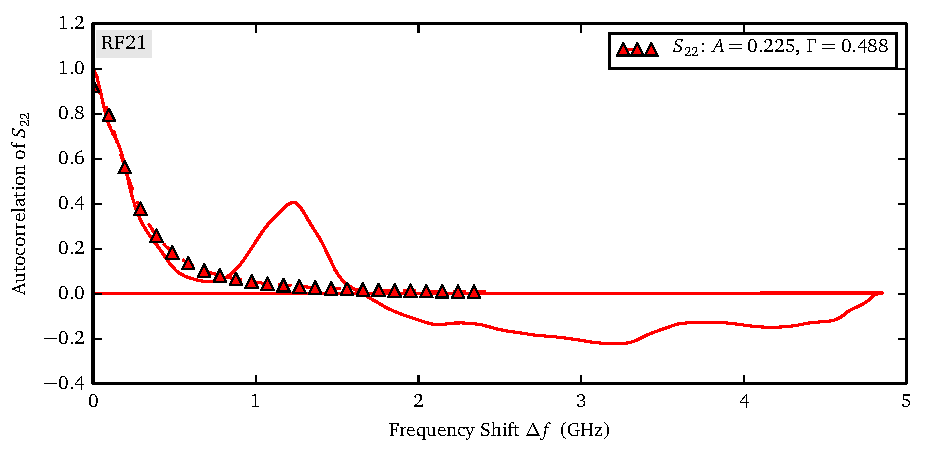
\includegraphics{figs/active/RF21-autoCorrelation.pdf}
 \caption[Autocorrelation of the experimental $S_{22}$ trace for the RF21 fibre-antenna]
 		{Autocorrelation of the experimental $S_{22}$ trace for the RF21 fibre-antenna.}
 \label{fig:active.lcx.rf21autocorrelation}
\end{figure}

\paragraph{RF27 and RF29}
As we can see from Table \ref{tab:active.antennae.rfxx-parameters}, these two antennae
are rather similar. It is thus not surprising that their $S$-parameters
show similar behaviour (compare Figures \ref{fig:active.lcx.rf27sParameters} and
\ref{fig:active.lcx.rf29sParameters}). Their small differences can be explained
away by the experimental variability of both the metal deposition and window
sizing protocols, as they have identical specifications.

Notice the quick decay of the autocorrelation function of the reflection 
coefficients, $S_{11}$ and $S_{22}$. If it were not for the hint of
regularity present in the autocorrelation function of $S_{12}$, 
it could be swiftly concluded that both antennae show chaotic scattering.
In any case, the lack of periodicity in the signals seems to indicate 
that the dip is not due to the geometry of the fibre-antenna. 

\begin{figure}
 \centering
 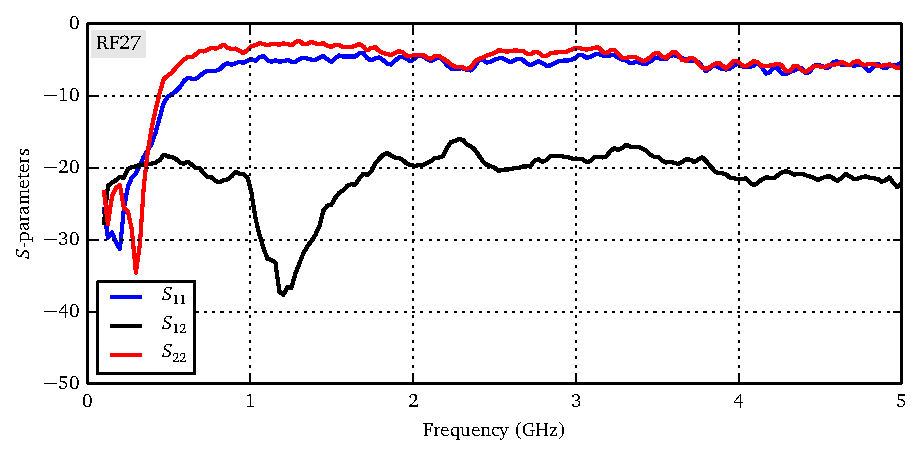
\includegraphics{figs/active/RF27-sParameters.pdf}
 \caption[Experimental $S$-parameter traces for the RF27 fibre-antenna]
 		{Experimental $S$-parameter traces for the RF27 fibre-antenna.}
 \label{fig:active.lcx.rf27sParameters}
\end{figure}

\begin{figure}
 \centering
 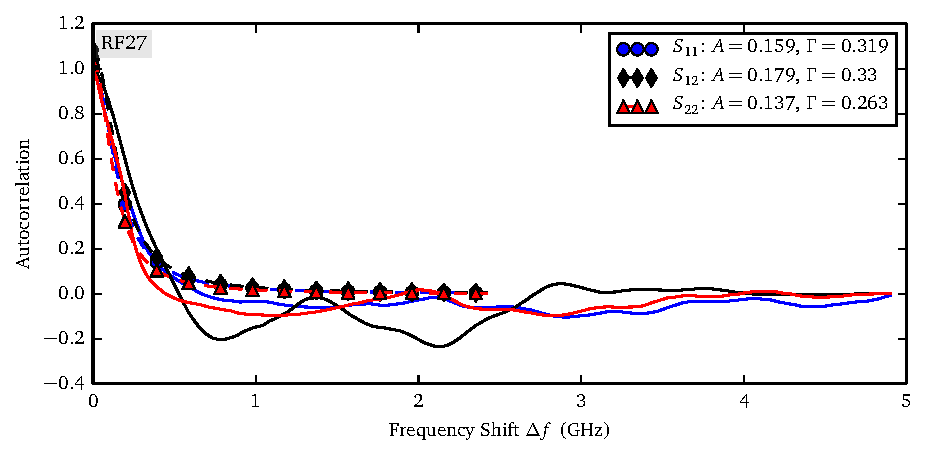
\includegraphics{figs/active/RF27-autoCorrelation.pdf}
 \caption[Autocorrelation of the experimental $S$-parameter traces for the RF27 fibre-antenna]
 		{Autocorrelation of the experimental $S$-parameter traces for the RF27 fibre-antenna.}
 \label{fig:active.lcx.rf27autocorrelation}
\end{figure}


\begin{figure}
 \centering
 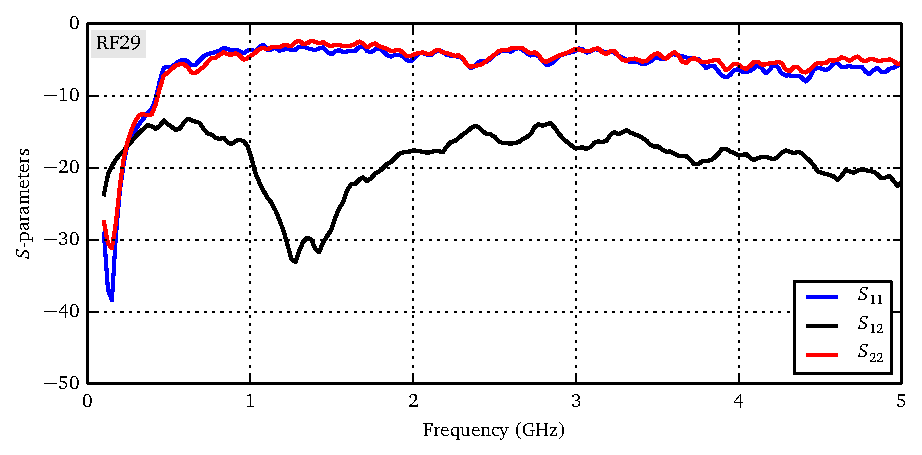
\includegraphics{figs/active/RF29-sParameters.pdf}
 \caption[Experimental $S$-parameter traces for the RF29 fibre-antenna]
 		{Experimental $S$-parameter traces for the RF29 fibre-antenna.}
 \label{fig:active.lcx.rf29sParameters}
\end{figure}

\begin{figure}
 \centering
 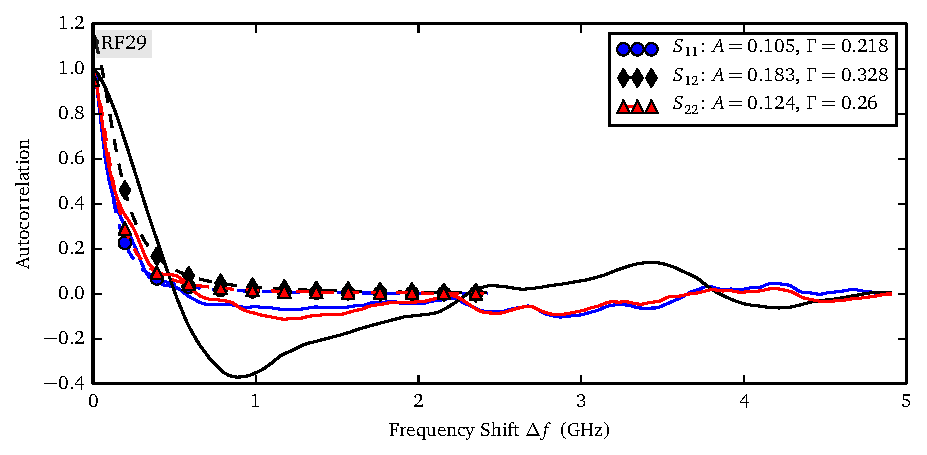
\includegraphics{figs/active/RF29-autoCorrelation.pdf}
 \caption[Autocorrelation of the experimental $S$-parameter traces for the RF29 fibre-antenna]
 		{Autocorrelation of the experimental $S$-parameter traces for the RF29 fibre-antenna.}
 \label{fig:active.lcx.rf29autocorrelation}
\end{figure}

\paragraph{RF33}
The RF33 fibre-antenna, the final antenna produced, is the most mature
one in terms of experimental protocol and is therefore most
worthy of study. Notice that the baseline for this fibre is 
higher than that of the other fibres. The dips also show lower quality,
although it is possible to make the LCX operate as an antenna
at some of the frequency dips. Specifically, there is a dip at
$f\sim2.6\,\unit{GHz}$, which is close to our requirements. 
There is however, an increase in the reflection coefficients
at this frequency, hinting that the antenna might not be 
efficient at that frequency. There seems to be a repetition 
of the trace at every $2\,\unit{GHz}$. 

The autocorrelation of the trace of $S_{22}$ shows a strong
periodic component, which we have isolated by taking the 
FFT of the signal. 
Figure \ref{fig:active.lcx.rf33fft} shows the intensity
of the FFT transform. To see if the periodic components corresponded
to particular lengths in the system, we converted the associated
wavelengths to frequencies. 
The fundamental mode of infinite \gls{lcx} \cite{WAN2001} is
  \begin{equation}
   f_1 = \frac{c}{\left(S_z+d_z\right)\left(\sqrt{\epsilon_\text{Si}}+1\right)} \sim 1.6\,\unit{GHz}.
  \end{equation}
The frequency associated with the optical and the actual lengths of the window
are
  \begin{align*}
   l_\text{opt}	&= \frac{c}{S_z\sqrt{\epsilon_\text{Si}}} \sim 4.5\,\unit{GHz}	\\
   l_\text{phy}	&= \frac{c}{S_z} \sim 8\,\unit{GHz}.
  \end{align*}

Nothing thus far seems to explain the periodic properties of the 
experimental $S_{22}$ trace, although it might just be that 
$f_1$ depends on the sizes $d_L$ and $d_R$ and what we see is
the fundamental mode of our quasi-LCX. 

\begin{figure}
 \centering
 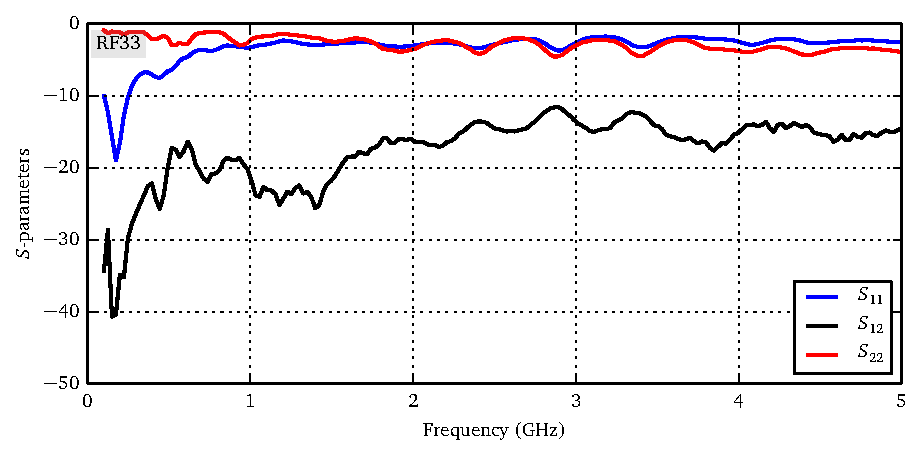
\includegraphics{figs/active/RF33-sParameters.pdf}
 \caption[Experimental $S$-parameter traces for the RF33 fibre-antenna]
 		{Experimental $S$-parameter traces for the RF33 fibre-antenna.}
 \label{fig:active.lcx.rf33sParameters}
\end{figure}

\begin{figure}
 \centering
 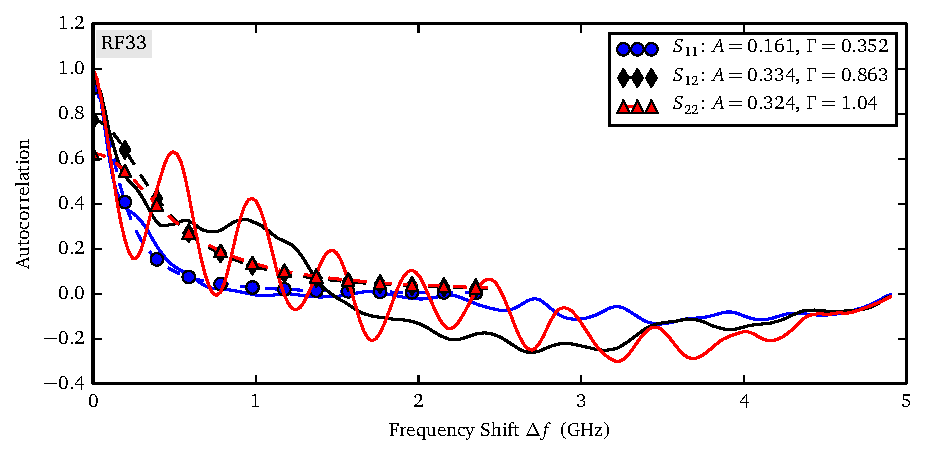
\includegraphics{figs/active/RF33-autoCorrelation.pdf}
 \caption[Autocorrelation of the experimental $S$-parameter traces for the RF33 fibre-antenna]
 		{Autocorrelation of the experimental $S$-parameter traces for the RF33 fibre-antenna.}
 \label{fig:active.lcx.rf33autocorrelation}
\end{figure}

\begin{figure}
 \centering
 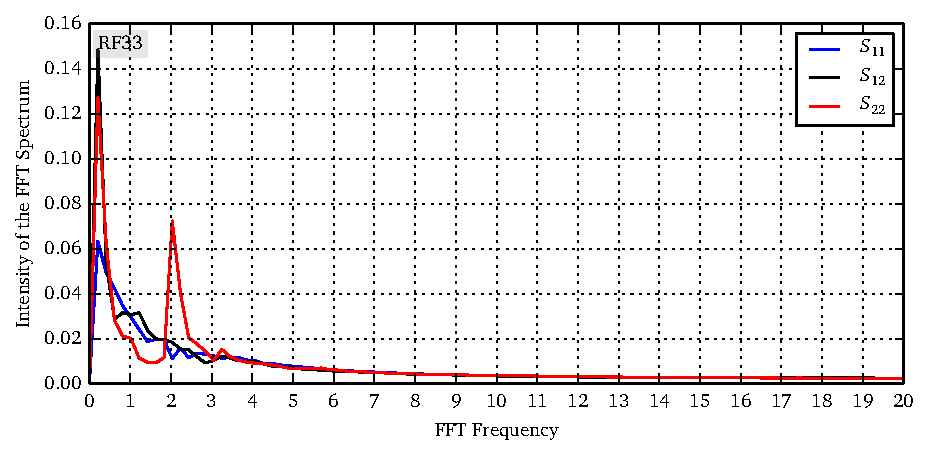
\includegraphics{figs/active/RF33-fft.pdf}
 \caption[FFT spectrum of the autocorrelation functions of the $S$-parameters of the RF33 fibre-antenna]
 		{FFT spectrum of the autocorrelation functions of the $S$-parameters of the RF33 fibre-antenna.}
 \label{fig:active.lcx.rf33fft}
\end{figure}


\subsubsection{Comparison with Simulation Results}
The specifications of each RFXX was based on the numerical simulation
of the antennae. However, once they were built, it became clear the 
numerical modeling did not correlate well with the experimental
realizations. As we will see, the experimental traces rarely possess
the same features as the numerical ones and the far-field patterns 
do not match. 

The main cause for such poor agreement between theory and experiment
was hypothesized to be related to the metallic layers. As discussed
above, the experimental method the group used did not allow for any
control over the thickness of metal deposited, and did not guarantee
its mechanical properties nor its chemical ones. In other words, 
the layers could be grainy and contain impurities. The former was taken
into account directly in the HFSS software, as the ``Layered Impedance
Boundary Conditions'' module allows for inhomogeneities in the surfaces.
The author of this essay thus tried to model the effects of impurities 
on the conductivity and the effect of the resulting small thicknesses
of the layers. The next section details the modeling efforts.  

\paragraph{Preliminary Results}
Because of its easily interpretable traces and of its (at the time)
quality, the RF21 fibre is the one we analyze. Figure
\ref{fig:active.lcx.rf21sParameters-sim} shows both the experimental traces
and the numerically predicted ones. Note that this simulation did not contain
any effective boundary conditions, but assumed that the silver layers had a 
constant $2\,\unit{\mu m}$ thickness. We can see transmission-line behaviour
in the $S_{12}$ parameter, as the wave is transmitted without much loss
regardless of frequency. Clearly, this model does not represent reality
well. Removing the silver layers and replacing them by effective boundary
conditions does not solve the problem, as is shown in Figure 
\ref{fig:active.lcx.rf21sParameters-concSweep}. 

\begin{figure}
 \centering
 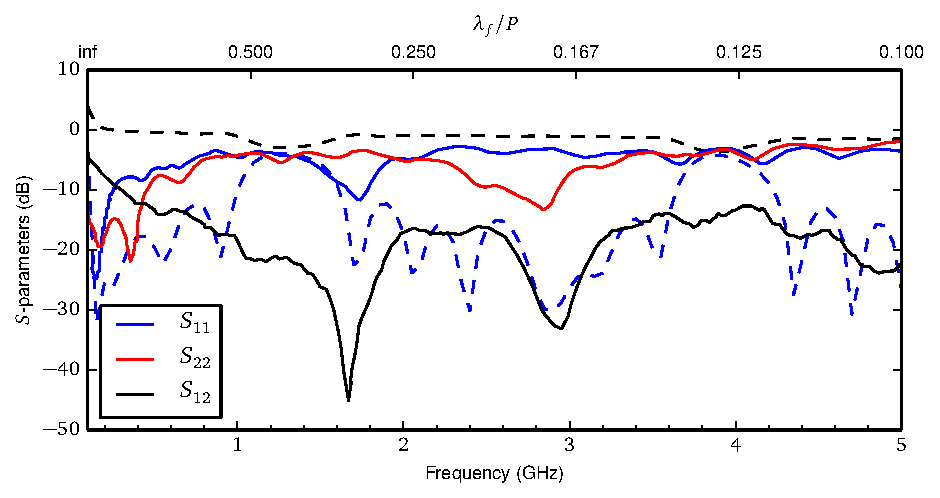
\includegraphics[width=\textwidth]{figs/active/sParametersRF21.pdf}
 \caption[$S$-parameters of the RF21 fibre design]
 		{$S$-parameters of the RF21 fibre design. The full lines represent
	  	the experimental data while the dotted lines represent the simulation data.
	  	The top $x$ axis shows the $S$-parameters as a function of the ratio of the 
	  	vacuum wavelength $\lambda_f$ over the period of the windows $P$.}
 \label{fig:active.lcx.rf21sParameters-sim}
\end{figure}

\paragraph{Modeling the Effect ot Thin Metallic Layers}
AFM pictures (see Figure \ref{fig:active.lcx.AFM})  have suggested that the deposited
metal is in fact a mixture of silver and silver oxide. To evaluate
the effective conductivity of the mixture, we have used Bruggeman's model \cite{LAN1978}.
The model starts from a homogeneous medium, call it medium 1, 
of conductivity $\sigma_1$ and replaces spherical portions of this material 
by another one of conductivity $\sigma_2$. When this process is done, 
we are left with a inhomogeneous material with partial concentrations $\delta_i$
of each material. The effective conductivity $\sigma_e$ of the medium can be computed
using the relation (for an arbitrary number of materials)
  \begin{equation}
    \sum_i^n \delta_i \frac{\sigma_i-\sigma_e}{\sigma_i+(d-1)\sigma_e} =0 
  \end{equation}
where $\sum_i\delta_i=1$ and $d$ is the dimensionality of the system.
Solving for $\sigma_e$ in the case $n=2$ yields
  \begin{equation}
   (d-1)\sigma_e^2+\left[\left(d\delta_1-1\right)\sigma_1+\left(d\delta_2-1\right)\sigma_2\right]+\sigma_1\sigma_2=0.
  \end{equation}
The positive solution is, defining $q=\left(d\delta_1-1\right)\sigma_1+\left(d\delta_2-1\right)\sigma_2$
  \begin{equation}
   \label{eq:antenna:bruggeman}
   \sigma_e = \frac{1}{2d-2}\left[q+\sqrt{q^2+4(d-1)\sigma_1\sigma_2}\right].
  \end{equation}
Using this effective conductivity in \eqref{eq:active.antennae.thickGeneralEquations} yields 
the associated thicknesses. We use $d=3$ throughout.

\begin{figure}
 \centering
 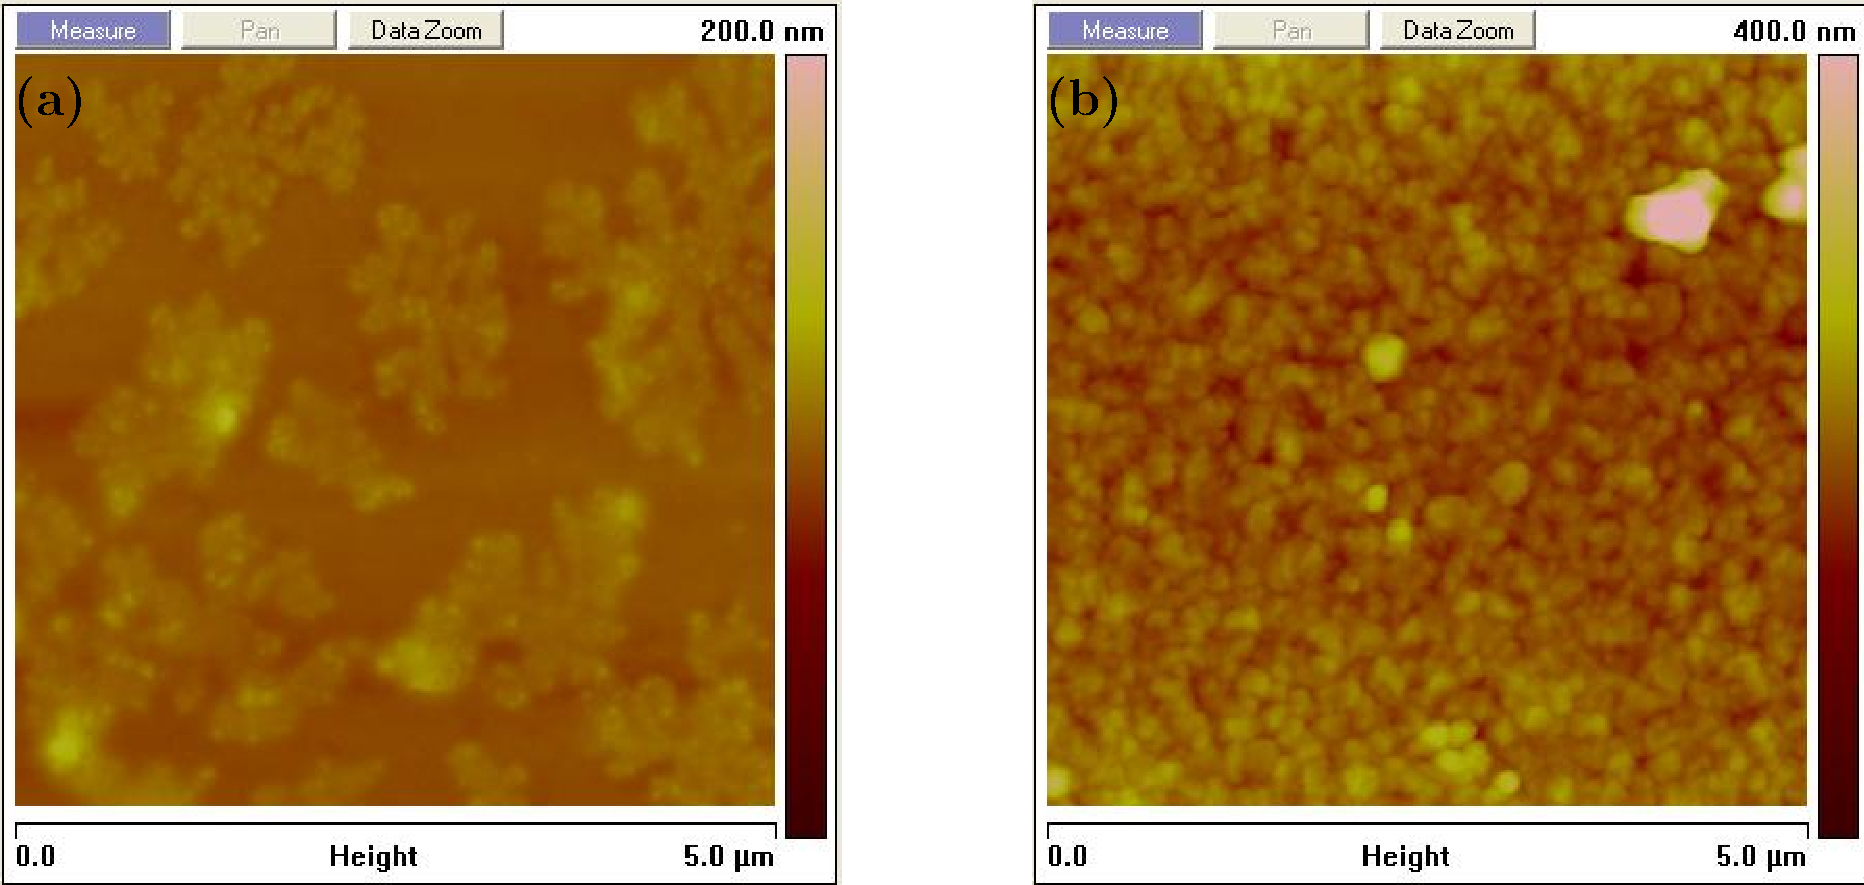
\includegraphics[width=0.8\textwidth]{figs/active/out/AFM.pdf}
 \caption[AFM pictures of silver deposited onto glass plates]
 		{AFM pictures of silver deposited onto glass plates. \textbf{(a)} Flakes of silver oxide seem to be forming onto the deposited
	  	silver layer. \textbf{(b)} Sample image showing the inhomogeneity of the
	  	silver layer.}
 \label{fig:active.lcx.AFM}
\end{figure}

It also came to light that the conductivity 
of thin metal films can be a function of their thicknesses. 
The state-of-the-art model to describe this dependence is the 
\textit{Fuchs-Sondheimer} model, which essentially computes the 
electron distribution in the metal as a function of its thickness. 
From Ohm's law, it is then trivial to obtain the value of the 
conductivity \cite{FUC1938,SON1952,PUR2007}. The general relationship
is
	\begin{multline}
		\frac{\sigma_F}{\sigma_0} = 
			1-\frac{3(1-p)}{8\kappa}\\+\frac{3}{4\kappa}\left(1-p\right)^2
			\sum_{\nu=1}^\infty p^{\nu-1}
			\left\{
				\int_{\kappa\nu}^\infty\frac{e^{-\xi}}{\xi}d\xi\left(\kappa^2\nu^2-\frac{\kappa^4\nu^4}{12}\right)
				+e^{-\kappa\nu}\left(\frac{1}{2}-\frac{5\kappa\nu}{6}-\frac{\kappa^2\nu^2}{12}+\frac{\kappa^3\nu^3}{12}\right)	
			\right\}
	\end{multline}
where $\kappa=t/\lambda_0$ where $\lambda_0$ is the mean free path of the electrons in the metal and
$t$ the thickness of the sample. The parameter $p$ is the proportion of electrons that are reflected
elastically at the boundary. For rough edges, we expect the electrons to be scattered off randomly 
and thus $p\sim0$. Notice that the above expression is extremely unwieldy and yields to a highly
non-linear root search when substituted in \eqref{eq:active.antennae.thickGeneralEquations}. 
We will use the much more convenient form (valid for $\kappa\ll1$) \cite{FUC1938}
  \begin{equation}
      \sigma_F = \frac{\sigma_0}{1+\frac{3\lambda}{8t}\left(1-p\right)}
  \end{equation}
which leads to a simpler cubic equation for the thickness.
This model states that conductivity
diminishes as the thickness of the metallic layer gets smaller, 
as one would expect.

In Figure \ref{fig:antenna.thicknessRatios}, we show the changes
in the predicted conductivities and thicknesses of the silvers layers
if we take the Bruggeman and Fuchs-Sondheimer models into account. 
Given that the AFM pictures
show surface inhomogeneity, we assume diffuse scattering in 
the FS model ($p=0$). Both the changes in effective conductivities
and thicknesses cover an order of magnitude, which should lead
to changes in the $S$-parameters. 


\begin{figure}
  \centering
  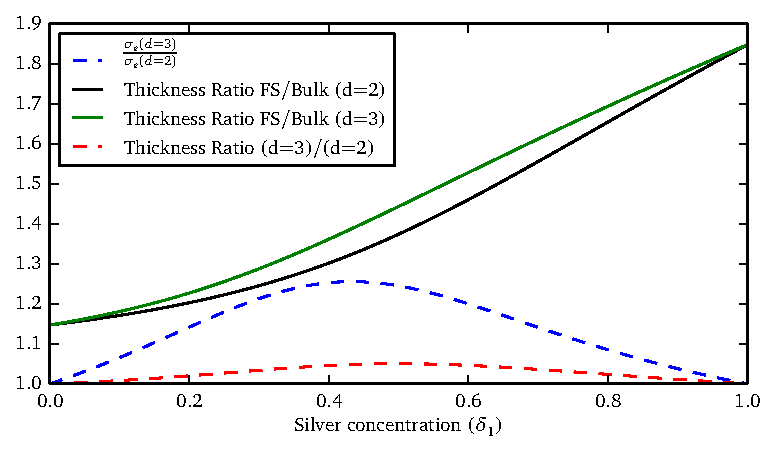
\includegraphics[width=0.9\textwidth]{figs/active/comparisonThickness.pdf}
  \caption[Thickness and conductivity as a function of the silver concentration]
	  {Conductivities and thicknesses predicted by the Bruggeman and Fuchs-Sondheimer
	  models as a function of the silver concentration, $\delta_1$. Conductivity increases
	  as $\delta_1$ increases and the thickness correspondingly decreases.}
  \label{fig:antenna.thicknessRatios}
\end{figure}

We have simulated the RF21 fibre using Bruggeman's model
for the effective conductivity and with values
of $\delta_1\in\{0,1\}$ and $d=3$ in \eqref{eq:antenna:bruggeman}.
After obtaining the simulated $S_\text{11}$ parameter of the fibre,
we compared it to the experimentally obtained one using the Pearson
correlation coefficient. For two samples $\{X_i\}$ and 
$\{Y_i\}$, it is defined as
  \begin{equation}
    r = \frac{\sum_i^n\left(X_i-\left\langle X\right\rangle\right)\left(Y_i-\left\langle Y\right\rangle\right)}
	     {\sqrt{\sum_i^n\left(X_i-\left\langle X\right\rangle\right)^2}\sqrt{\sum_i^n\left(Y_i-\left\langle Y\right\rangle\right)^2}}.
  \end{equation}
From the definition, we see that the simultaneous linear transformations $X_i\rightarrow b+aX_i$ and $Y_i\rightarrow d+cY_1$
do not change the value of the Pearson coefficient. This means that even if the two samples
do not have the same normalization or are shifted by a constant amount, the correlation 
will stay the same. As such, the Pearson correlation measures the degree at which 
both samples are linearly related. 

Figure \ref{fig:active.lcx.rf21sParameters-sim} shows the experimental and simulated
$S_{11}$ parameter. At first look, it might seem like the general form 
of the curves are similar, but our quantitative analysis shows
that that would be wrong. To make sure that our simulation data was not simply
shifted in frequency due to a small error in the geometry, we have
also calculated the correlation for a shifted dataset 
\footnote{To do so, we simply right-shifted the arrays containing
the simulation data and removed the data that fell outside the frequency range 
of the experimental data.}. This changes
the Pearson correlation because we must elide some of the experimental
and simulation data to do so. Figure \ref{fig:antenna.shiftCorrelation}
shows our results. We see that there are little to no correlation
between the simulation data and the experimental data with $r\in\{-0.04,0.05\}$, 
and this is true for all silver concentrations. Although it is not shown, were
also performed with the Fuchs-Sondheimer model: the $S$-parameters did not
vary appreciably from those shown here.

\begin{figure}
 \centering
 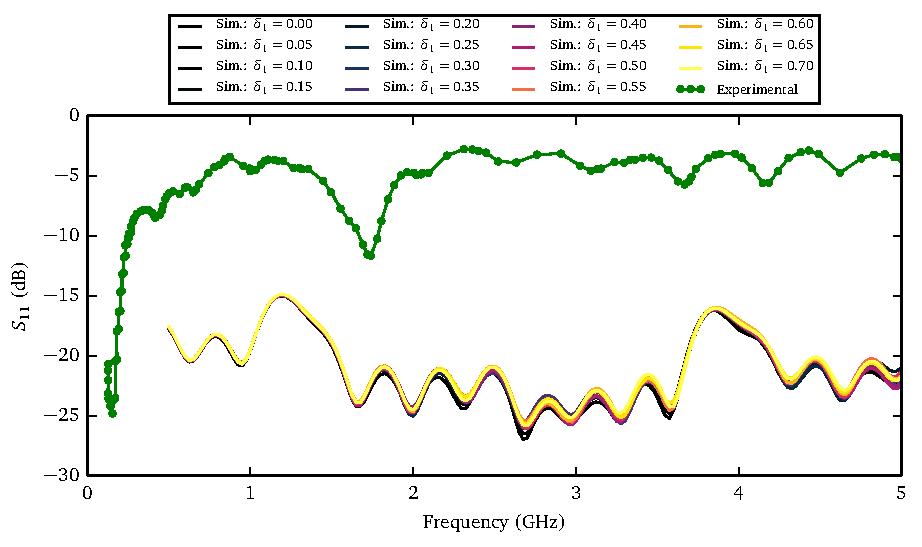
\includegraphics[width=0.8\textwidth]{figs/active/sParameters-concSweepS11.pdf}
 \caption[Experimental and simulated $S_{11}$ parameter for the RF21 fibre]
	 {Experimental and simulated $S_{11}$ parameter for the RF21 fibre.}
 \label{fig:active.lcx.rf21sParameters-concSweep}
\end{figure}

\begin{figure}
 \centering
 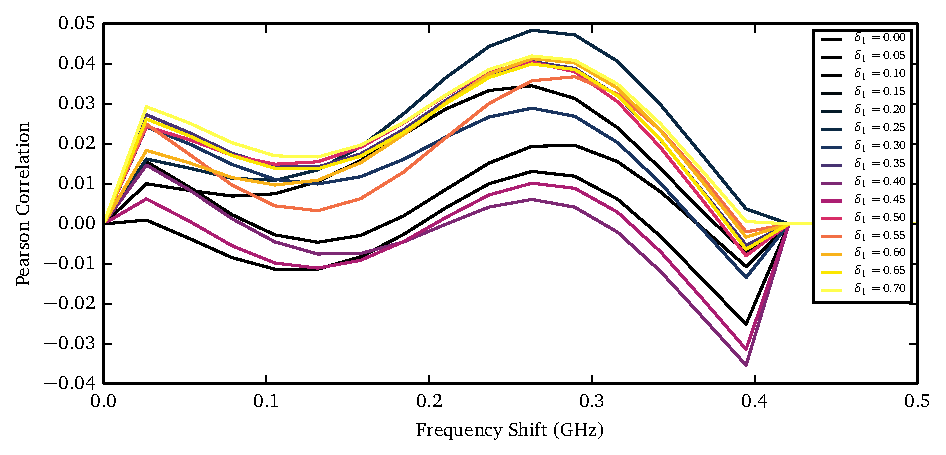
\includegraphics[width=0.8\textwidth]{figs/active/shiftCorrelationS11.pdf}
 \caption{Pearson correlation coefficient as a function of the frequency
	  shift of the data.}
 \label{fig:antenna.shiftCorrelation}
\end{figure}

We unfortunately conclude this section by noting that the above phenomena
are not sufficient to explain the lack of correlation between the experimental
and simulation datasets. The models do predict dramatically different properties
for the metallic layers, but it seems that this does not affect the $S$-parameters
all that much. One explanation is that the effect of the surface inhomogeneities
are \textit{not} taken into account when computing the thicknesses; they are only
accounted for \textit{a posteriori} in the FEM software. By using an
\textit{ab initio} model to compute the effects of randomly distributed inhomogeneities
on the base conductivity $\sigma_0$ of the metallic layers \cite{CUR2012}, one could obtain a better
estimate of the thicknesses and possibly a better fit between the experimental and simulated datasets.

We can see, however, that while of the details of the $S$-parameters are not well reproduced, some
dips appear both in experimental and simulated traces. The irregular scattering, due to the experimental
variations of the geometry, could account for the suppression of some dips and the possible shifts. 
However, it is difficult to predict \textit{a priori} which ones will be suppressed and which ones will
be shifted, as we do not have ``robustness'' information. 